\chapter{Experimental Results}\label{ch:expRes}

In the following chapter the different variants of the RLS and the (1+1) EA are now analysed empirically for the best algorithm depending on the input.
Additionally for most lemmas from the previous chapters there are also tests if they actually hold in practice.

\section{Code}
The complete java code used for all empirical studies is available on \href{https://github.com/Err404NameNotFound/PartitionSolvingWithEAs}{GitHub}.
\subsection{The Algorithms}
All different variants of the RLS function more or the less the same. They start with an initial random value and then optimise this one value in the loop. The loop can be summarised like this:
\begin{enumerate}
      \item generate a number k of bits to be flipped (algorithm specific)
      \item flip k random bits
      \item evaluate fitness of the mutated individual
      \item replace old value with new value if new value is better
      \item repeat if not optimal
\end{enumerate}
The (1+1) EA variants behave differently on the first impression as they flip bit each bit independently with probability $c/n$.
This can be seen as $n$ independent Bernoulli trials with probability $c/n$.
The amount of bits that are flipped is therefore binomial distributed and the algorithm can be implemented exactly as the versions of the RLS. The same holds for the $pmut$ operator which generates a number $k$ from a powerlaw distribution and then flips $k$ bits.
This leads to only one implementation of a partition solving algorithm which is not only given the input array of numbers but also a generator for the amount of bits to be flipped in each step.
The random values for the amount of bits to be flipped are generated according to this table:

\begin{tabular}[h]{c c}
      Algorithm & Returned value                                                                          \\
      \hline
      RLS       & 1                                                                                       \\
      RLS-N$_k$ & $y \in \{1,\dots,k\}$ with probability $\frac{\binom{n}{y}}{\sum_{i=1}^k \binom{n}{i}}$ \\
      RLS-R$_K$ & uniform random value $y \in \{1,\dots,k\}$                                              \\
      (1+1) EA  & binomial distributed value from \textasciitilde$B(n,c/n)$                               \\
      pMut      & powerlaw distributed value from \textasciitilde$D^\beta_n$                              \\
\end{tabular}



\begin{algorithm}[bt]
      \caption{\textsc{GenericPartitionSolver}}\label{alg:genericPartition}

      % Some settings
      \DontPrintSemicolon %dontprintsemicolon
      \SetFuncSty{textsc}

      % The algorithm
      \BlankLine
      choose x uniform random from ${\{0,1\}}^n$\;
      \While{$x$ not optimal}
      {
      $x' \leftarrow x$\;
      $k \leftarrow \text{kGenerator.generate()}$\;
      flip $k$ uniform random bits of $x'$\;
      {
      \If{$f(x') \le f(x)$}
      {
            $x \leftarrow x'$\;
      }
      }
      }
\end{algorithm}

\subsection{Random number generation}

Java only provides a random number generator for uniform distributed values for any integer interval or random double values $\in \left[0, 1\right)$.
For this project this does not suffice as for an efficient way of implementing the (1+1) EA or simply for generating a binomial distributed input another random number generator is needed.
One of the needed distributions is a binomial distribution.
The simplest way to generate a number \textasciitilde$B(m,p)$ would be to run a loop $m$ times and add 1 to the generated number if a uniform random value $\in \left[0, 1\right)$ is less than $p$.
This works perfectly fine and generates numbers according to the distribution.
With low values for p this approach is rather inefficient and especially for values of $p=1/m$.
The expected value in this case is 1 but generating a random number takes time $\mathcal{O}(m)$.
Another more efficient way was implemented by StackOverflow user \href{https://stackoverflow.com/users/2166798/pjs}{pjs} on \href{https://stackoverflow.com/questions/23561551/a-efficient-binomial-random-number-generator-code-in-java}{stackoverflow} inspired by Devroyes method introduced in~\cite{devroye2006nonuniform}.
This method has an expected running time of $\mathcal{O}(mp)$ which is equal to the expected value of the distribution.
For the case of $p=1/m$ this runs in expected constant time in comparison to $\mathcal{O}(m)$ for the naive way.
This number generation was also used for the implementation of the (1+1) EA instead of running a for loop in every step.

\begin{algorithm}[h]
      \caption{\textsc{Binomial random number generator}}\label{alg:binomialRNG}

      % Some settings
      \DontPrintSemicolon %dontprintsemicolon
      \SetFuncSty{textsc}
      $q \leftarrow \ln(1.0 - p)$\;
      $x \leftarrow 0$\;
      $sum \leftarrow 0$\;
      \While{true}
      {
      $sum \leftarrow sum +\ln(\text{random()}) / (n - x)$\; \tcp{random() generates a random value $\in \left[0, 1\right)$}
      \If{sum < q}
      {
            return $x$\;
      }
      $x \leftarrow x + 1$\;
      }
\end{algorithm}

The next generator needed is for geometric distributed values.
This generator is only necessary for the generation of geometric distributed inputs but not for the algorithms.
The easiest way to generate geometric distributed values is the naive way:
generating a uniform random value until the generated value is at least as big as $p$.
The expected running time of this algorithm is equal to the expected value of the distribution $1/p$.
So this method is comparably effective to the approach used for binomial random number generation.

\begin{algorithm}[h]
      \caption{\textsc{Geometric random number generator}}\label{alg:geometricRNG}

      % Some settings
      \DontPrintSemicolon %dontprintsemicolon
      \SetFuncSty{textsc}
      $sum \leftarrow 0$\; \tcp{random() generates a random value $\in \left[0, 1\right)$}
      \While{\text{random()} $\ge$ q}
      {
            $sum \leftarrow sum+1$\;
      }
      return $sum$\;
\end{algorithm}

The last generator needed is for powerlaw distributed values.
This generator is in contrast to the geometric number generator needed for both the algorithm with the $pmut_\beta$ mutation operator and for generating inputs.
This implementation is also from stackoverflow. The user \href{https://stackoverflow.com/users/52738/gnovice}{gnovice} provided the following formula on \href{https://stackoverflow.com/questions/918736/random-number-generator-that-produces-a-power-law-distribution}{this} page on stackoverflow:
\[
      x = {[(b^{n+1} - q^{n+1})*y + a^{n+1}]}^{1/(n+1)}
\]
$a$ is the lower bound, $b$ the upper bound, $n$ the parameter of the distribution and $y$ the number generated uniform random $\in \left[0, 1\right)$.
The idea behind the formula and the formula itself is explained in a \href{https://mathworld.wolfram.com/RandomNumber.html}{mathworld} page.


\section{Do inputs have perfect partitions?}
\subsection{Binomial Inputs}

Lemma~\ref{lemma:BinomialSolvable} is only valid for larger n.
In practice the bound is much smaller depending on the expected value of a single value.
Another factor deciding how likely an input is to have a perfect partition is if n is even or odd.
To determine the influence of all factors multiple experiments were conducted.
The goal of the first experiment was to determine the influence of the array size to the input having a perfect partition and the fact if n is even or odd.
So for every possible combination of $p \in \{0.1, 0.2, \dots , 0.8, 0.9\}, m \in \{10,100,1000,10^4,10^5\} \text{ and } n \in \{2,3,4,\dots,19,20\}$ 1000 randomly generated inputs of size $n$ were tested for a perfect partition.
Due to the small values for $n$ it was possible to brute force the results in a short amount of time.
The results are visualised in figure~\ref{fig:firstBinPercentage} to figure~\ref{fig:lastBinPercentage}.
On the x-axis is the size of the input and on the y-axis the percentage of inputs that had a perfect partition.
The different graphs in each figure resemble the different values of p used for generating the inputs.
The graph for $p=0.1$ resembles the percentage of inputs that had a perfect partition with values generated from the distribution \textasciitilde$B(m,0.1)$ with $m$ being dependent on the figure.
For figure~\ref{fig:firstBinPercentage} $m$ has the value 10.\newline
It is easy to see that for small inputs sizes it is relevant if n is even or odd for higher expected values as all curves in figure~\ref{fig:lastBinPercentage} oscillate between 0\% and 100\% for $n\ge14$.
For uneven inputs the probability of a perfect partition decreases much more drastically with m as for even inputs because the expected value of a single number increases with m.
If all values are much higher the small differences between the values can no longer even out the fact of one set having more elements than the other.
The oscillation therefore increases with increasing m.
For $n=20$ all 1000 inputs had a perfect partition for every combination of $p$ and $m$ but for $n=19$ only combinations where $mp\le300$ holds had at least one input a perfect partition.
For expected values of up to $10^5$ it seems to be almost granted that an input of length 20 has a perfect partition if it is binomial distributed.
Even for only 12 binomial generated values more than 50\% of the inputs had a perfect partition (see figure~\ref{fig:lastBinPercentage}).
Another visible effect is the decreasing percentage with rising p.
This may be a direct result of the value chosen for p but can also be an indirect result as the value for p changes the expected value for a constant m.
The expected value may have an influence on the number of perfect partitions because it influences the highest value of the input.
For uniform distributed inputs Borgs showed that the coefficient of \#bits needed to encode the max value/$n$ has a huge impact on the number of perfect partitions~\cite{borgs2001phase}.
For a coefficient < 1 the probability of a perfect partition tends to 1 and for a coefficient > 1 it tends to 0.
This was only proven for the uniform distributed input, but it might also hold for a binomial distributed input.
This leads to the second experiment.

\begin{figure}[h]
      \centering
      \begin{minipage}[b]{0.45\textwidth}
            \caption{Percentage of Binomial inputs with perfect partitions for m = 10}
            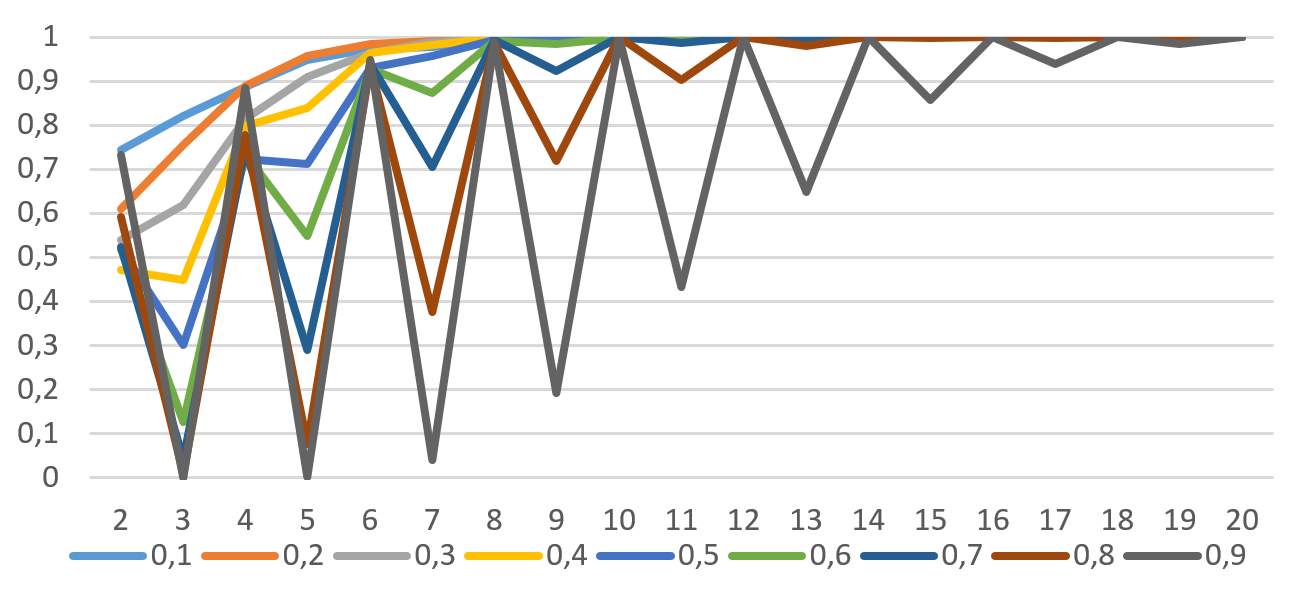
\includegraphics[width=\textwidth]{figures/images/solvabilityOfInputs/binomial_Input_Solvable_m10.png}\label{fig:firstBinPercentage}
      \end{minipage}
      \hspace{0.75cm}
      \begin{minipage}[b]{0.45\textwidth}
            \caption{Percentage of Binomial inputs with perfect partitions for m = 100}
            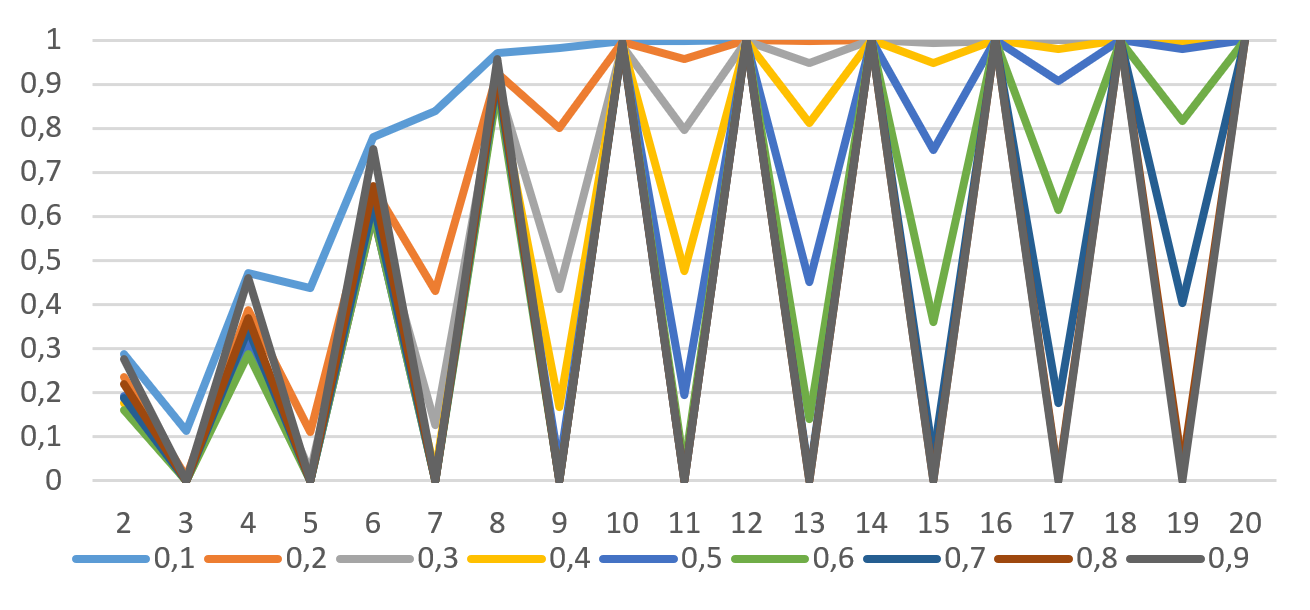
\includegraphics[width=\textwidth]{figures/images/solvabilityOfInputs/binomial_Input_Solvable_m100.png}
      \end{minipage}
\end{figure}

\begin{figure}[h]
      \centering
      \begin{minipage}[b]{0.45\textwidth}
            \caption{Percentage of Binomial inputs with perfect partitions for m = 1000}
            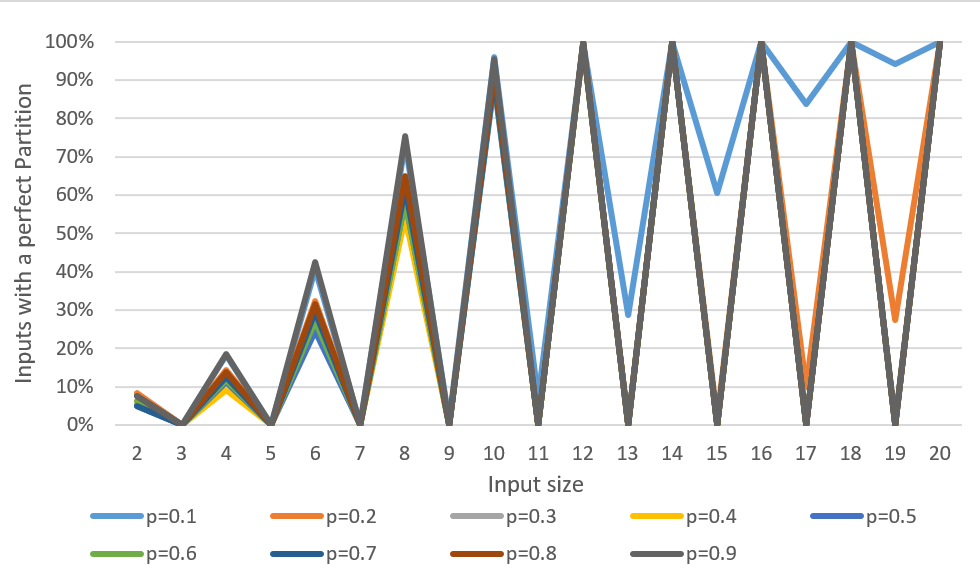
\includegraphics[width=\textwidth]{figures/images/solvabilityOfInputs/binomial_Input_Solvable_m1000.png}
      \end{minipage}
      \hspace{0.75cm}
      \begin{minipage}[b]{0.45\textwidth}
            \caption{Percentage of Binomial inputs with perfect partitions for m = 10000}
            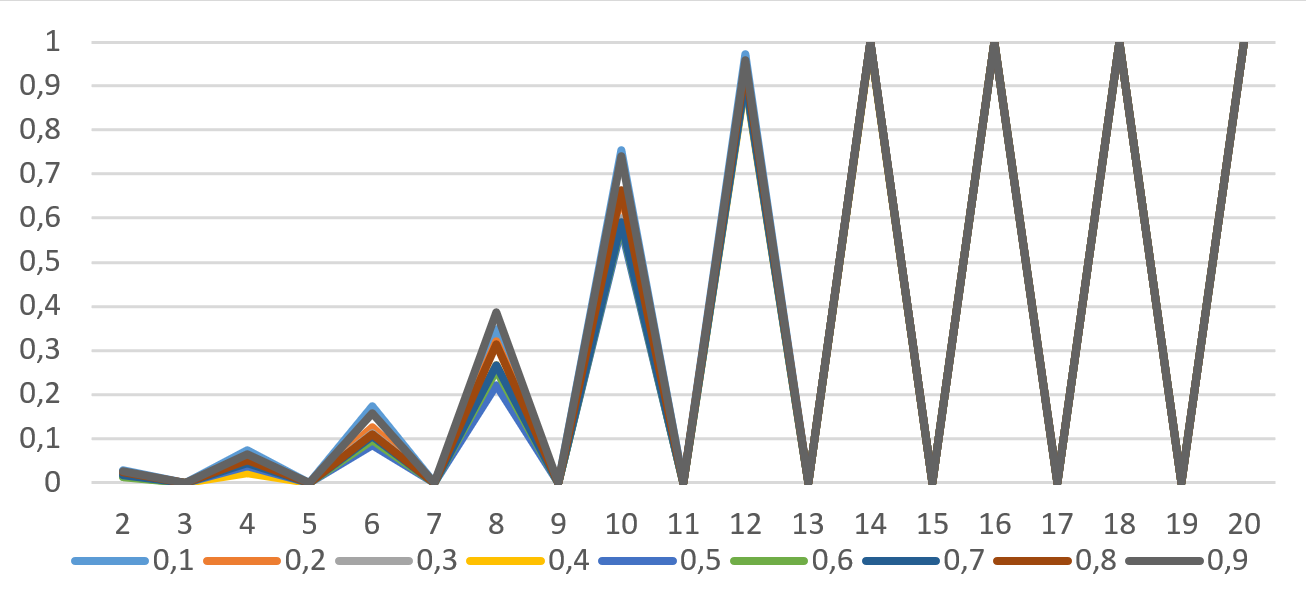
\includegraphics[width=\textwidth]{figures/images/solvabilityOfInputs/binomial_Input_Solvable_m10000.png}
      \end{minipage}
\end{figure}

\begin{figure}[h]
      \caption{Percentage of Binomial inputs with perfect partitions for m = 100000}
      \centering
      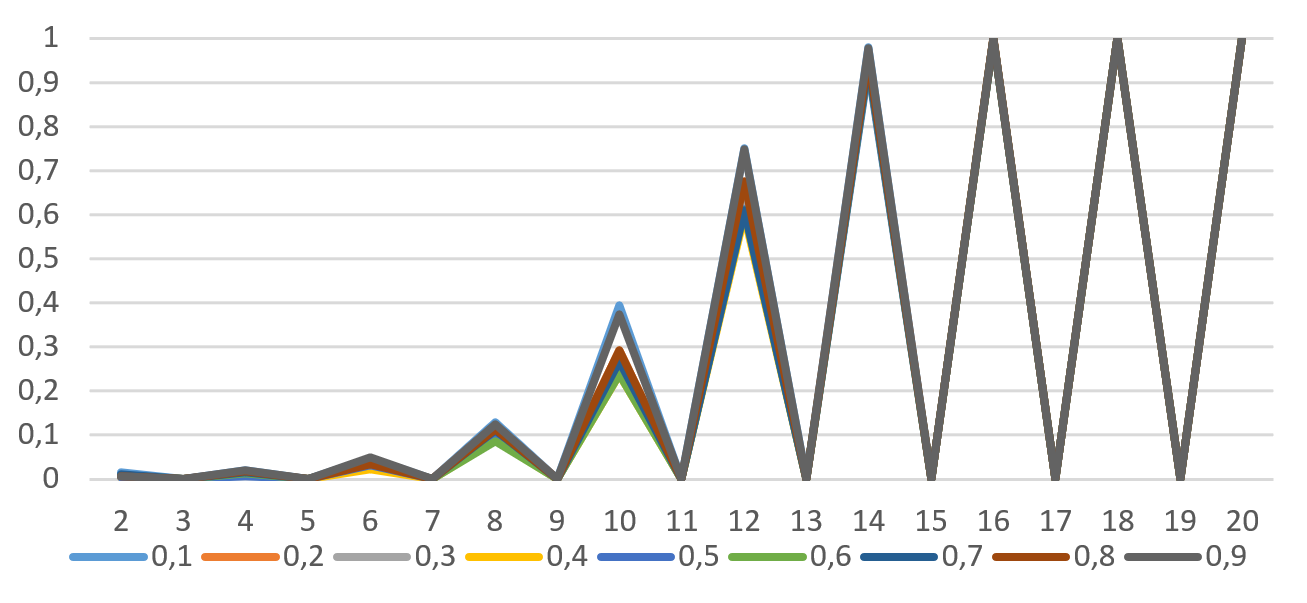
\includegraphics[width=0.45\textwidth]{figures/images/solvabilityOfInputs/binomial_Input_Solvable_m100000.png}\label{fig:lastBinPercentage}
\end{figure}


In the second experiment the inputs were generated a bit differently.
Here the goal was to keep the expected value fixed for any combination of $p$ and $n$ and set the value of $m$ to $e/p$ for all $e \in \{10, 20, 30, 40, 50, 100, 200, 500, 1000, 2000, 5000, 10000, 50000\}$ so that $E(X)=mp=e/p\cdot p=e$.
With this setup the influence of the expected value is almost isolated from the other parameters.
The probability is still linked to $p$ as $p$ also influences the variance $mp(1-p)$.
By looking at figure~\ref{fig:firstBinPercentage2} to figure~\ref{fig:lastBinPercentage2} it seems as if the value of $p$ has a much smaller influence than the expected value.
For a fixed expected value and a fixed input size a higher value for $p$ seems to only slightly increase the percentage of inputs with a perfect partition.
The expected value influences the percentage significantly more.
For $p=0.1, n=14$ the value decreases from 100\% at $E(X)=10$ to below 20\% at $E(X)=50000$.
For $p=0.9$ the percentage only drops below 50\% but still decreases by a factor of 2.

\begin{figure}[h]
      \centering
      \begin{minipage}[b]{0.45\textwidth}
            \caption{Percentage of Binomial inputs with perfect partitions for p = 0.1}
            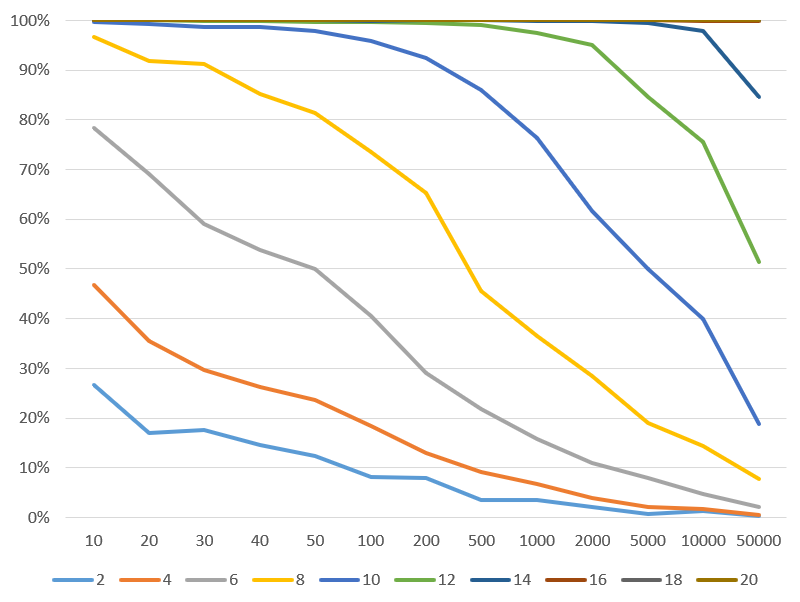
\includegraphics[width=\textwidth]{figures/images/solvabilityOfInputs/solvability0_1.png}\label{fig:firstBinPercentage2}
      \end{minipage}
      \hspace{0.75cm}
      \begin{minipage}[b]{0.45\textwidth}
            \caption{Percentage of Binomial inputs with perfect partitions for p = 0.2}
            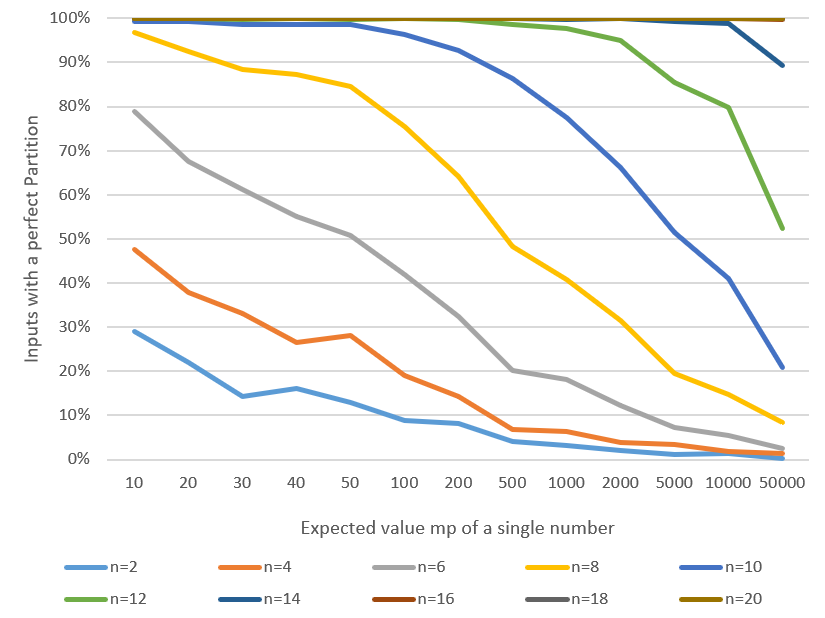
\includegraphics[width=\textwidth]{figures/images/solvabilityOfInputs/solvability0_2.png}
      \end{minipage}
\end{figure}


% \begin{figure}[h]
%       \centering
%       \begin{minipage}[b]{0.45\textwidth}
%             \caption{Percentage of Binomial inputs with perfect partitions for p = 0.3}
%             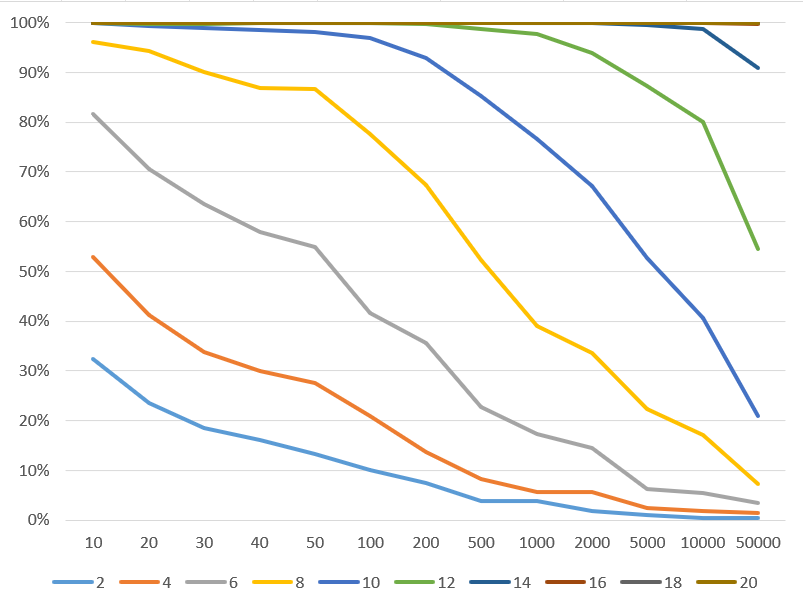
\includegraphics[width=\textwidth]{figures/images/solvabilityOfInputs/solvability0_3.png}
%       \end{minipage}
%       \hspace{0.75cm}
%       \begin{minipage}[b]{0.45\textwidth}
%             \caption{Percentage of Binomial inputs with perfect partitions for p = 0.4}
%             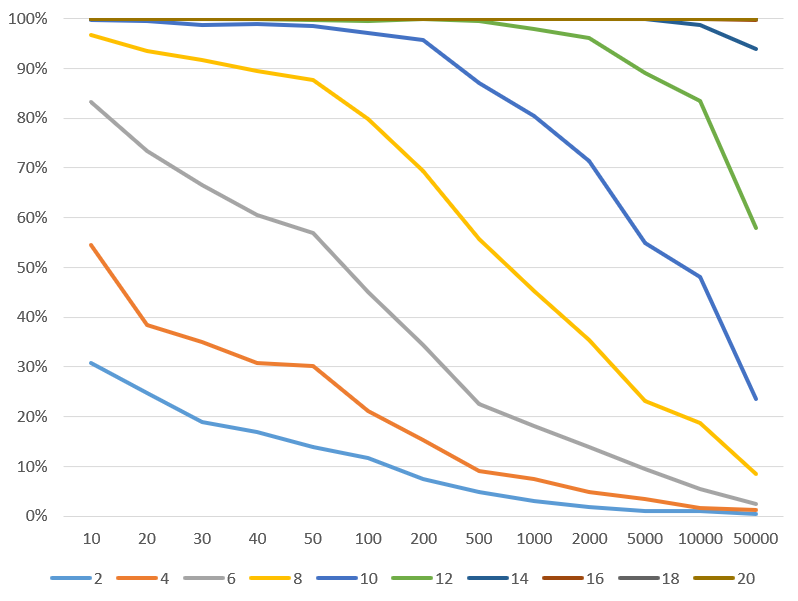
\includegraphics[width=\textwidth]{figures/images/solvabilityOfInputs/solvability0_4.png}
%       \end{minipage}
% \end{figure}


\begin{figure}[h]
      \centering
      \begin{minipage}[b]{0.45\textwidth}
            \caption{Percentage of Binomial inputs with perfect partitions for p = 0.5}
            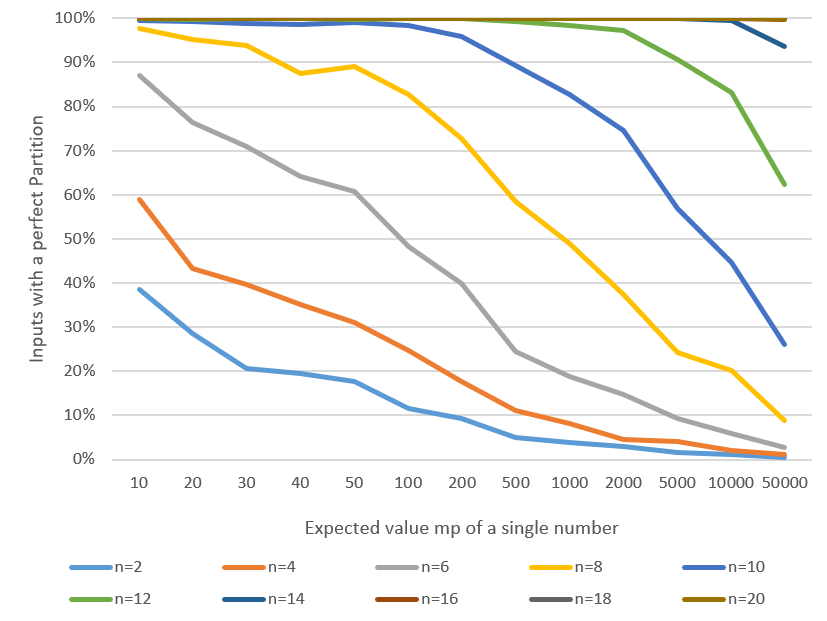
\includegraphics[width=\textwidth]{figures/images/solvabilityOfInputs/solvability0_5.png}
      \end{minipage}
      \hspace{0.75cm}
      \begin{minipage}[b]{0.45\textwidth}
            \caption{Percentage of Binomial inputs with perfect partitions for p = 0.9}
            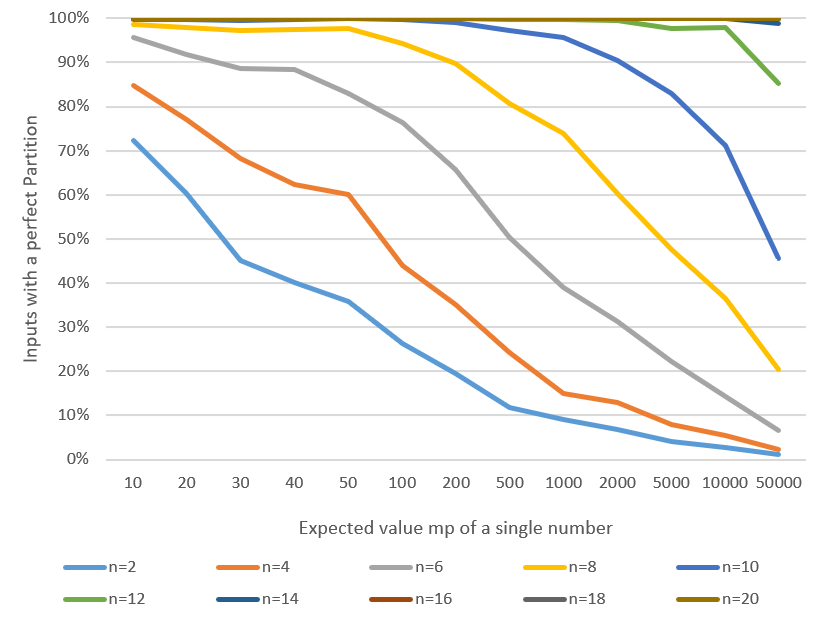
\includegraphics[width=\textwidth]{figures/images/solvabilityOfInputs/solvability0_9.png}\label{fig:lastBinPercentage2}
      \end{minipage}
\end{figure}

The last experiment showed that for $n=20$ 1000/1000 inputs had a perfect partition. This raised the question of how the amount of perfect partition changes with changing values for $m, p, n$.
Figure~\ref{fig:firstBinSolCount} to figure~\ref{fig:lastBinSolCount} show the amount of perfect partitions a binomial distribution \textasciitilde$B(m,p$) has.
For these figures 10,000 random binomial inputs with the given values for $m$ and $p$ were generated.
Each input was then tested for the amount of perfect partitions it has.
The method was again brute force due to the small input sizes.
After all runs the averages values were combined in the given figures.
The value of $p$ is dependent on the picture and each value of $m \in \{10,100,1000,10000\}$ has its own graph within the figure.
The x-axis is the size of the input and the y-axis the amount of perfect partitions the input has.
Notice that all graphs have a y-axis with a logarithmic scale.
Since the graphs are all linear the actual values rise exponentially.
The number of perfect partition is mostly multiplied by a factor between 3 and 4 when the input size increases by 2.

\begin{figure}[h]
      \centering
      \begin{minipage}[b]{0.45\textwidth}
            \caption{Amount of perfect partitions for $p=0.1$}
            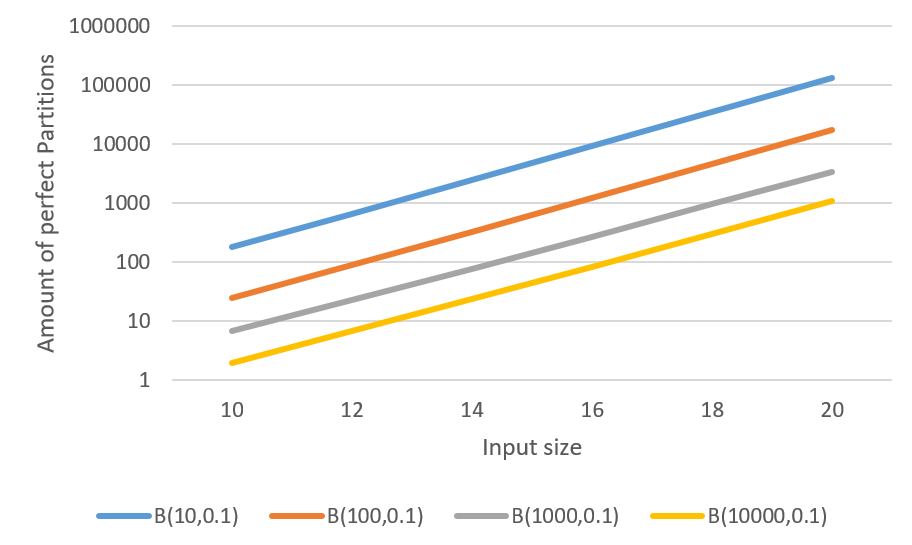
\includegraphics[width=\textwidth]{figures/images/solvabilityOfInputs/perfectPartitionCount-p0_1.png}\label{fig:firstBinSolCount}
      \end{minipage}
      \hspace{0.75cm}
      \begin{minipage}[b]{0.45\textwidth}
            \caption{Amount of perfect partitions for $p=0.9$}
            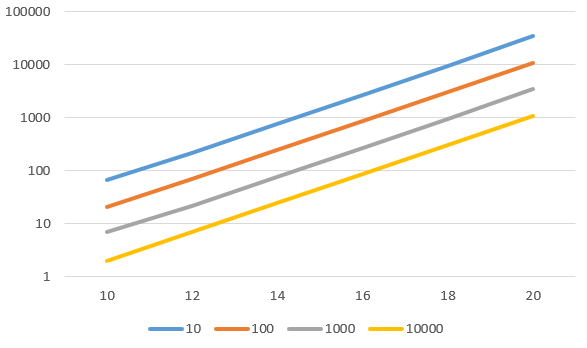
\includegraphics[width=\textwidth]{figures/images/solvabilityOfInputs/perfectPartitionCount-p0_9.png}
      \end{minipage}
\end{figure}

\begin{figure}[h]
      \centering
      \begin{minipage}[b]{0.45\textwidth}
            \caption{Amount of perfect partitions for $p=0.2$}
            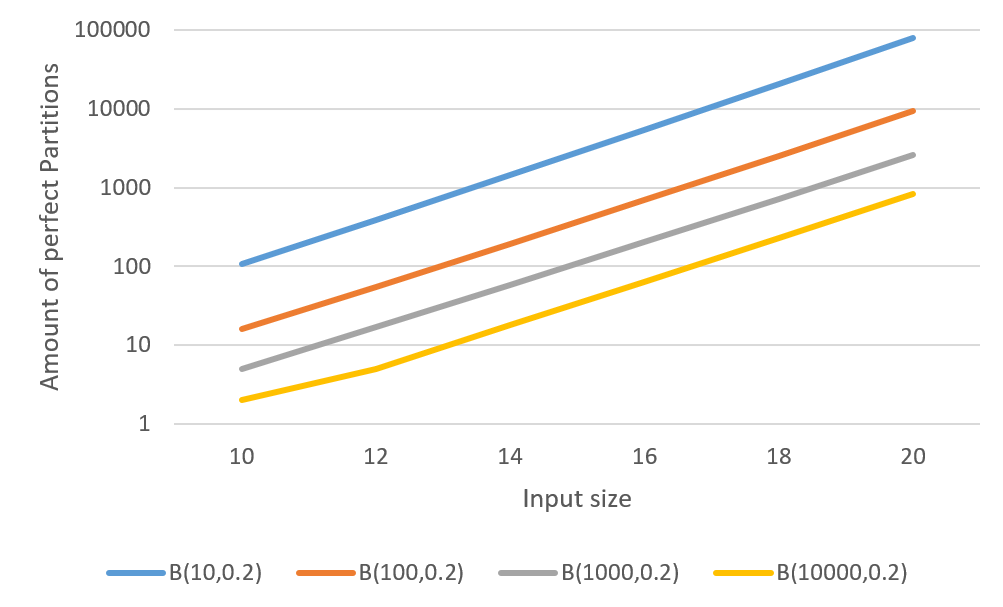
\includegraphics[width=\textwidth]{figures/images/solvabilityOfInputs/perfectPartitionCount-p0_2.png}
      \end{minipage}
      \hspace{0.75cm}
      \begin{minipage}[b]{0.45\textwidth}
            \caption{Amount of perfect partitions for $p=0.5$}
            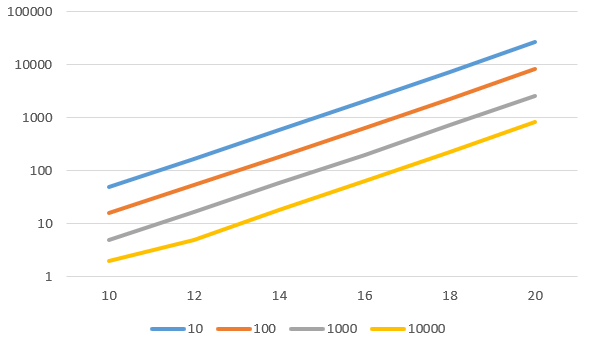
\includegraphics[width=\textwidth]{figures/images/solvabilityOfInputs/perfectPartitionCount-p0_8.png}\label{fig:lastBinSolCount}
      \end{minipage}
\end{figure}

The higher the value of $m$ the closer the curves of $p$ and $1-p$ get.
For $m=1000$ and $m=10000$ the values are almost the same for every input size.
% As in this case $m$ was not defined as $e/p$ with some values for $e$ but instead some values directly for $m$, the influence of the expected values distorts the image for the lower values of $m$.
For $p=0.1, m=10$ an input with expected values of 1 seems to much more likely to have a perfect partition than an input with expected value $10\cdot0.9=9$.
With growing $m$ this has less impact.
% Figure~\ref{fig:additionalBinSolCount} shows that for equal expected values the average amount of perfect partitions is the same for $p$ and $1-p$.
% Here this fact even holds for the smaller values of $m$.

% \begin{figure}[h]
%       \caption{Amount of perfect partitions for $p=0.1$ and $p=0.9$}
%       \centering
% 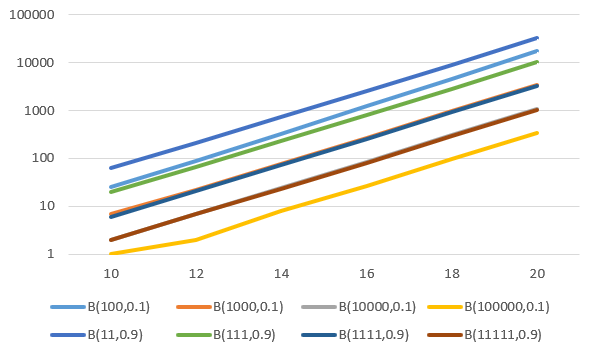
\includegraphics[width=0.45\textwidth]{figures/images/solvabilityOfInputs/perfectPartitionCount-p0_1Andp0_9_2.png}\label{fig:additionalBinSolCount}
% \end{figure}

So the binomial input should be easy to solve due to the exponential number of perfect partitions.
It might be harder for the smaller values of $n$ as there are only a few perfect partitions.
Due to the small number of total possibilities it should still be easy to solve for the small values of $n$ as long as the RSH is not stuck in a local optimum.
The number of iterations might be high in terms of the big-O notation but should still be small in the absolute value.
% BEGIN RESULTS

\section{Binomial distributed values}
This input is similar to the mixed input from the last subsection.
For this distribution the values are not chosen uniform random from one of the base distributions, but instead a value from every distribution is chosen and added together.
Hence the name overlapped distribution.
For this input the step limit was increased to $100\cdot n \ln n$.
The comparison with the step limit $10\cdot n \ln(n)$ is contained in the last subsubsection which compares the best variants.

\begin{figure}[h]
      \caption{Distribution of an overlapped input with \textasciitilde$U(1,999)$, \textasciitilde$B(1000,0.1)$, \textasciitilde$Geo(0.01)$, powerlaw dist with $\beta=-1.25$}
      \centering
      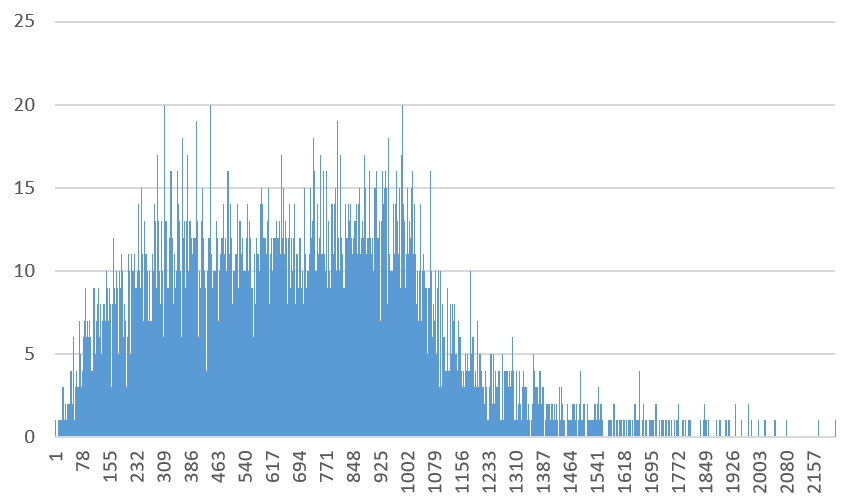
\includegraphics[width=0.7\textwidth]{figures/images/numberGenerator/overlapped.png}\label{fig:overlappedDistExample}
\end{figure}

Figure~\ref{fig:overlappedDistExample} looks completely different from figure~\ref{fig:mixedDistExample}.
No value is generated more than 20 times as opposed to the maximum amount of 350 for the mixed distribution.
In this figure no distribution is clearly visible.

The used distributions were \textasciitilde$U(1,49999)$, \textasciitilde$B(10000,0.1)$, \textasciitilde$Geo(0.001)$, powerlaw distribution with $\beta=-1.25$.
\subsection{RLS Comparison}
The following table lists the results for the RLS for inputs that are chosen from a powerlaw distribution with $\beta=-2.75$.


\makebox[\linewidth]{
\begin{tabular}{lp{3cm}p{6cm}p{6cm}}
\begin{tabular}[h]{cccccccc}
algo type&            \RLSN&     \RLSR&     \RLSR&     \RLSN&     \RLSR&     \RLSN&       RLS\\
algo param&             b=2&       s=3&       s=4&       b=3&       s=2&       b=4&         -\\
avg mut/change&       2.000&     1.996&     2.476&     3.000&     1.502&     4.000&     1.000\\
avg mut/step&         2.000&     2.000&     2.500&     3.000&     1.500&     4.000&     1.000\\
\hline
total avg count&     83,118&   104,748&   105,513&   112,223&   114,486&   121,927& 2,443,567\\
avg eval count&      83,118&   104,748&   105,513&   112,223&   114,486&   121,927&    45,834\\
max eval count&     778,110& 1,453,252&   898,974& 1,377,471&   915,268&   816,633&   485,275\\
min eval count&         197&       126&        45&       212&       271&       155&       128\\
\hline
fail ratio&           0.000&     0.000&     0.000&     0.000&     0.000&     0.000&     0.447\\
avg fail dif&             -&         -&         -&         -&         -&         -&         1\\
\end{tabular}
\end{tabular}
}


For these inputs the variants of the RLS perform differently to the binomial input.
The only similarity is the RLS being the worst as the RLS is the only algorithm that did not find an optimal solution for every input.
If the RLS did find an optimal solution in those 5 cases it would instead be the best RLS variant.
The other algorithms are ranked by the probability of flipping only one bit.
This means at first the three RLS-R variants from 2 to 3 to 4 and then the same for the RLS-N variants.
So it does seem like moving mostly one element at once is better for the geometric input in comparison to two elements for the binomial distribution.
In the 5 cases where the RLS did not find an optimal solution it was most likely stuck in a local optimum.

\subsection{(1+1) EA Comparison}
The first table again shows the results for parameter $\beta=-2.75$

\makebox[\linewidth]{
\begin{tabular}{lp{3cm}p{6cm}p{6cm}}
\begin{tabular}[h]{ccccccccc}
algo type&          (1+1) EA&   (1+1) EA&   (1+1) EA&   (1+1) EA&      (1+1) EA&   (1+1) EA&   (1+1) EA&   (1+1) EA\\
algo param&           3/n&     4/n&     2/n&     5/n&       -&    10/n&    50/n&   100/n\\
avg mut/change&     3.101&   3.968&   2.343&   4.859&   1.698&   9.732&  49.544&  99.494\\
avg mut/step&       2.999&   4.003&   2.002&   4.999&   1.001&   9.998&  49.998&  99.997\\
\hline
total avg count&      646&     701&     706&     857&   1,123&   1,508&   8,175&  15,485\\
avg eval count&       646&     701&     706&     857&   1,123&   1,508&   8,175&  15,485\\
max eval count&     5,346&   5,692&   3,415&   5,572&   7,001&  12,112&  52,831& 145,269\\
min eval count&        23&       4&      30&       9&      23&      14&      27&      69\\
\hline
fails&                  0&       0&       0&       0&       0&       0&       0&       0\\
fail ratio&         0.000&   0.000&   0.000&   0.000&   0.000&   0.000&   0.000&   0.000\\
avg fail dif&           -&       -&       -&       -&       -&       -&       -&       -\\
\end{tabular}
\end{tabular}
}


For the EA the result is also the inversion of the results for the OneMax equivalent.
The higher the mutation rate the better at least up to $n\le100$.
From mutation rate $p_m\le3/n$ the algorithm reaches the worst case at least once in 1000 runs.
If the algorithm did not manage to find an optimal solution the fitness was always the same.
So there was no run where any algorithm neither found a global nor the local optimum.
\subsection{pmut Comparison}
The first table again shows the results for parameter $\beta=-2.75$

\makebox[\linewidth]{
\scriptsize
\begin{tabular}{lp{3cm}p{6cm}p{6cm}}
\begin{tabular}[h]{m{2.5cm}m{0,40cm}m{0,40cm}m{0,40cm}m{0,40cm}m{0,40cm}m{0,40cm}m{0,40cm}m{0,40cm}m{0,40cm}m{0,40cm}m{0,40cm}m{0,40cm}m{0,40cm}m{0,40cm}m{0,40cm}m{0,40cm}m{0,40cm}m{0,40cm}}
\multicolumn{1}{c}{algo type}&\multicolumn{2}{c}{            pmut}&\multicolumn{2}{c}{     pmut}&\multicolumn{2}{c}{     pmut}&\multicolumn{2}{c}{     pmut}&\multicolumn{2}{c}{     pmut}&\multicolumn{2}{c}{     pmut}&\multicolumn{2}{c}{     pmut}&\multicolumn{2}{c}{     pmut}&\multicolumn{2}{c}{     pmut}\\
\multicolumn{1}{c}{algo param}&\multicolumn{2}{c}{           3.25}&\multicolumn{2}{c}{     3.00}&\multicolumn{2}{c}{     2.75}&\multicolumn{2}{c}{     2.50}&\multicolumn{2}{c}{     2.25}&\multicolumn{2}{c}{     2.00}&\multicolumn{2}{c}{     1.75}&\multicolumn{2}{c}{     1.50}&\multicolumn{2}{c}{     1.25}\\
\multicolumn{1}{c}{avg mut/change}&\multicolumn{2}{c}{      1.583}&\multicolumn{2}{c}{    1.737}&\multicolumn{2}{c}{    2.002}&\multicolumn{2}{c}{    2.423}&\multicolumn{2}{c}{    3.303}&\multicolumn{2}{c}{    5.830}&\multicolumn{2}{c}{   12.519}&\multicolumn{2}{c}{   30.910}&\multicolumn{2}{c}{   73.182}\\
\multicolumn{1}{c}{avg mut/step}&\multicolumn{2}{c}{        1.729}&\multicolumn{2}{c}{    1.934}&\multicolumn{2}{c}{    2.274}&\multicolumn{2}{c}{    2.895}&\multicolumn{2}{c}{    4.360}&\multicolumn{2}{c}{    8.452}&\multicolumn{2}{c}{   22.278}&\multicolumn{2}{c}{   70.532}&\multicolumn{2}{c}{  224.421}\\
\hline
\multicolumn{1}{c}{avg eval count}&\multicolumn{2}{c}{        540}&\multicolumn{2}{c}{      569}&\multicolumn{2}{c}{      594}&\multicolumn{2}{c}{      641}&\multicolumn{2}{c}{      712}&\multicolumn{2}{c}{      808}&\multicolumn{2}{c}{      967}&\multicolumn{2}{c}{    1,285}&\multicolumn{2}{c}{    2,081}\\
\multicolumn{1}{c}{max eval count}&\multicolumn{2}{c}{      3,110}&\multicolumn{2}{c}{    2,891}&\multicolumn{2}{c}{    3,504}&\multicolumn{2}{c}{    3,896}&\multicolumn{2}{c}{    5,152}&\multicolumn{2}{c}{    4,274}&\multicolumn{2}{c}{    5,610}&\multicolumn{2}{c}{    6,190}&\multicolumn{2}{c}{   14,984}\\
\multicolumn{1}{c}{min eval count}&\multicolumn{2}{c}{         22}&\multicolumn{2}{c}{        9}&\multicolumn{2}{c}{       36}&\multicolumn{2}{c}{       25}&\multicolumn{2}{c}{       28}&\multicolumn{2}{c}{       27}&\multicolumn{2}{c}{       27}&\multicolumn{2}{c}{       13}&\multicolumn{2}{c}{       33}\\
\hline
\multicolumn{1}{c}{fail ratio}&\multicolumn{2}{c}{          0.000}&\multicolumn{2}{c}{    0.000}&\multicolumn{2}{c}{    0.000}&\multicolumn{2}{c}{    0.000}&\multicolumn{2}{c}{    0.000}&\multicolumn{2}{c}{    0.000}&\multicolumn{2}{c}{    0.000}&\multicolumn{2}{c}{    0.000}&\multicolumn{2}{c}{    0.000}\\
\hline
\multicolumn{1}{c}{p-value}&&\multicolumn{2}{c}{0.0000}&\multicolumn{2}{c}{0.0000}&\multicolumn{2}{c}{0.0000}&\multicolumn{2}{c}{0.0000}&\multicolumn{2}{c}{0.0000}&\multicolumn{2}{c}{0.0000}&\multicolumn{2}{c}{0.0000}&\multicolumn{2}{c}{0.0000}\\
&&&&&&&&&&&&&&&&&&\end{tabular}
\end{tabular}
}


The ideal value for $\beta$ seems to be around -1.75 as the runtime increases for the two neighbour values.
Even the worst value still manages find an optimal solution within double the time of the best value.
The importance of the parameter is therefore not as important as for other inputs.
\subsection{Comparison of the best variants}
The first table again shows the results for parameter $\beta=-2.75$

\makebox[\linewidth]{
\begin{tabular}{lp{3cm}p{6cm}p{6cm}}
\begin{tabular}[h]{cccc}
algo type&            RLS&    pmut&      EA\\
algo param&             -&    3.25&       -\\
avg mut/change&     1.000&   1.287&   1.272\\
avg mut/step&       1.000&   1.729&   1.000\\
\hline
avg eval count&    91,171& 143,121& 231,082\\
max eval count&   153,143& 227,737& 446,942\\
min eval count&    65,783&  93,602& 165,818\\
\hline
fail ratio&         0.000&   0.000&   0.000\\
\end{tabular}
\end{tabular}
}


The results for this experiment are as expected.
All three algorithms find the optimal value within the time limit.
The RLS performs better than the (1+1) EA because it does only single bit flips.
The $pmut_{-3.25}$ perform better than the standard (1+1) EA although flipping more bits on average.
This is most likely cause by the few steps where $pmut$ flips many bits which increase the average.
But $pmut$ most likely chooses to flip only one bit more often as the (1+1) EA.

TODO insert comparison with multiple values of n.
\section{Geometric distributed values}
This input is similar to the mixed input from the last subsection.
For this distribution the values are not chosen uniform random from one of the base distributions, but instead a value from every distribution is chosen and added together.
Hence the name overlapped distribution.
For this input the step limit was increased to $100\cdot n \ln n$.
The comparison with the step limit $10\cdot n \ln(n)$ is contained in the last subsubsection which compares the best variants.

\begin{figure}[h]
      \caption{Distribution of an overlapped input with \textasciitilde$U(1,999)$, \textasciitilde$B(1000,0.1)$, \textasciitilde$Geo(0.01)$, powerlaw dist with $\beta=-1.25$}
      \centering
      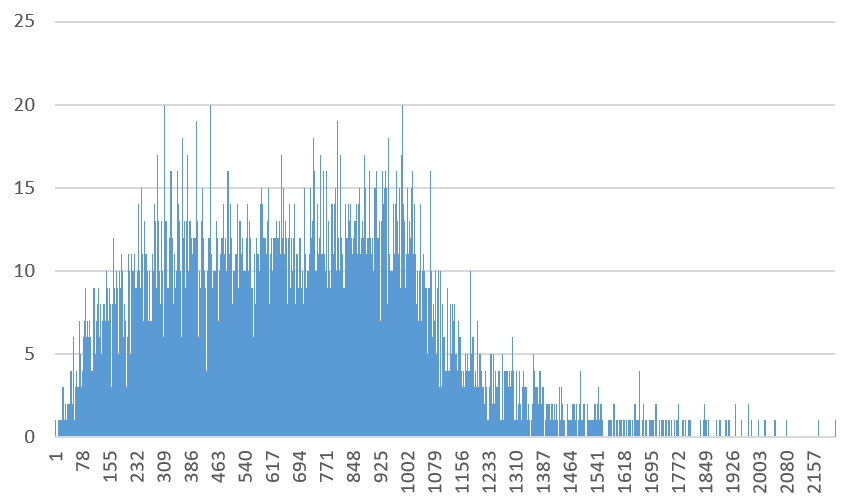
\includegraphics[width=0.7\textwidth]{figures/images/numberGenerator/overlapped.png}\label{fig:overlappedDistExample}
\end{figure}

Figure~\ref{fig:overlappedDistExample} looks completely different from figure~\ref{fig:mixedDistExample}.
No value is generated more than 20 times as opposed to the maximum amount of 350 for the mixed distribution.
In this figure no distribution is clearly visible.

The used distributions were \textasciitilde$U(1,49999)$, \textasciitilde$B(10000,0.1)$, \textasciitilde$Geo(0.001)$, powerlaw distribution with $\beta=-1.25$.
\subsection{RLS Comparison}
The following table lists the results for the RLS for inputs that are chosen from a powerlaw distribution with $\beta=-2.75$.


\makebox[\linewidth]{
\begin{tabular}{lp{3cm}p{6cm}p{6cm}}
\begin{tabular}[h]{cccccccc}
algo type&            \RLSN&     \RLSR&     \RLSR&     \RLSN&     \RLSR&     \RLSN&       RLS\\
algo param&             b=2&       s=3&       s=4&       b=3&       s=2&       b=4&         -\\
avg mut/change&       2.000&     1.996&     2.476&     3.000&     1.502&     4.000&     1.000\\
avg mut/step&         2.000&     2.000&     2.500&     3.000&     1.500&     4.000&     1.000\\
\hline
total avg count&     83,118&   104,748&   105,513&   112,223&   114,486&   121,927& 2,443,567\\
avg eval count&      83,118&   104,748&   105,513&   112,223&   114,486&   121,927&    45,834\\
max eval count&     778,110& 1,453,252&   898,974& 1,377,471&   915,268&   816,633&   485,275\\
min eval count&         197&       126&        45&       212&       271&       155&       128\\
\hline
fail ratio&           0.000&     0.000&     0.000&     0.000&     0.000&     0.000&     0.447\\
avg fail dif&             -&         -&         -&         -&         -&         -&         1\\
\end{tabular}
\end{tabular}
}


For these inputs the variants of the RLS perform differently to the binomial input.
The only similarity is the RLS being the worst as the RLS is the only algorithm that did not find an optimal solution for every input.
If the RLS did find an optimal solution in those 5 cases it would instead be the best RLS variant.
The other algorithms are ranked by the probability of flipping only one bit.
This means at first the three RLS-R variants from 2 to 3 to 4 and then the same for the RLS-N variants.
So it does seem like moving mostly one element at once is better for the geometric input in comparison to two elements for the binomial distribution.
In the 5 cases where the RLS did not find an optimal solution it was most likely stuck in a local optimum.

\subsection{(1+1) EA Comparison}
The first table again shows the results for parameter $\beta=-2.75$

\makebox[\linewidth]{
\begin{tabular}{lp{3cm}p{6cm}p{6cm}}
\begin{tabular}[h]{ccccccccc}
algo type&          (1+1) EA&   (1+1) EA&   (1+1) EA&   (1+1) EA&      (1+1) EA&   (1+1) EA&   (1+1) EA&   (1+1) EA\\
algo param&           3/n&     4/n&     2/n&     5/n&       -&    10/n&    50/n&   100/n\\
avg mut/change&     3.101&   3.968&   2.343&   4.859&   1.698&   9.732&  49.544&  99.494\\
avg mut/step&       2.999&   4.003&   2.002&   4.999&   1.001&   9.998&  49.998&  99.997\\
\hline
total avg count&      646&     701&     706&     857&   1,123&   1,508&   8,175&  15,485\\
avg eval count&       646&     701&     706&     857&   1,123&   1,508&   8,175&  15,485\\
max eval count&     5,346&   5,692&   3,415&   5,572&   7,001&  12,112&  52,831& 145,269\\
min eval count&        23&       4&      30&       9&      23&      14&      27&      69\\
\hline
fails&                  0&       0&       0&       0&       0&       0&       0&       0\\
fail ratio&         0.000&   0.000&   0.000&   0.000&   0.000&   0.000&   0.000&   0.000\\
avg fail dif&           -&       -&       -&       -&       -&       -&       -&       -\\
\end{tabular}
\end{tabular}
}


For the EA the result is also the inversion of the results for the OneMax equivalent.
The higher the mutation rate the better at least up to $n\le100$.
From mutation rate $p_m\le3/n$ the algorithm reaches the worst case at least once in 1000 runs.
If the algorithm did not manage to find an optimal solution the fitness was always the same.
So there was no run where any algorithm neither found a global nor the local optimum.
\subsection{pmut Comparison}
The first table again shows the results for parameter $\beta=-2.75$

\makebox[\linewidth]{
\scriptsize
\begin{tabular}{lp{3cm}p{6cm}p{6cm}}
\begin{tabular}[h]{m{2.5cm}m{0,40cm}m{0,40cm}m{0,40cm}m{0,40cm}m{0,40cm}m{0,40cm}m{0,40cm}m{0,40cm}m{0,40cm}m{0,40cm}m{0,40cm}m{0,40cm}m{0,40cm}m{0,40cm}m{0,40cm}m{0,40cm}m{0,40cm}m{0,40cm}}
\multicolumn{1}{c}{algo type}&\multicolumn{2}{c}{            pmut}&\multicolumn{2}{c}{     pmut}&\multicolumn{2}{c}{     pmut}&\multicolumn{2}{c}{     pmut}&\multicolumn{2}{c}{     pmut}&\multicolumn{2}{c}{     pmut}&\multicolumn{2}{c}{     pmut}&\multicolumn{2}{c}{     pmut}&\multicolumn{2}{c}{     pmut}\\
\multicolumn{1}{c}{algo param}&\multicolumn{2}{c}{           3.25}&\multicolumn{2}{c}{     3.00}&\multicolumn{2}{c}{     2.75}&\multicolumn{2}{c}{     2.50}&\multicolumn{2}{c}{     2.25}&\multicolumn{2}{c}{     2.00}&\multicolumn{2}{c}{     1.75}&\multicolumn{2}{c}{     1.50}&\multicolumn{2}{c}{     1.25}\\
\multicolumn{1}{c}{avg mut/change}&\multicolumn{2}{c}{      1.583}&\multicolumn{2}{c}{    1.737}&\multicolumn{2}{c}{    2.002}&\multicolumn{2}{c}{    2.423}&\multicolumn{2}{c}{    3.303}&\multicolumn{2}{c}{    5.830}&\multicolumn{2}{c}{   12.519}&\multicolumn{2}{c}{   30.910}&\multicolumn{2}{c}{   73.182}\\
\multicolumn{1}{c}{avg mut/step}&\multicolumn{2}{c}{        1.729}&\multicolumn{2}{c}{    1.934}&\multicolumn{2}{c}{    2.274}&\multicolumn{2}{c}{    2.895}&\multicolumn{2}{c}{    4.360}&\multicolumn{2}{c}{    8.452}&\multicolumn{2}{c}{   22.278}&\multicolumn{2}{c}{   70.532}&\multicolumn{2}{c}{  224.421}\\
\hline
\multicolumn{1}{c}{avg eval count}&\multicolumn{2}{c}{        540}&\multicolumn{2}{c}{      569}&\multicolumn{2}{c}{      594}&\multicolumn{2}{c}{      641}&\multicolumn{2}{c}{      712}&\multicolumn{2}{c}{      808}&\multicolumn{2}{c}{      967}&\multicolumn{2}{c}{    1,285}&\multicolumn{2}{c}{    2,081}\\
\multicolumn{1}{c}{max eval count}&\multicolumn{2}{c}{      3,110}&\multicolumn{2}{c}{    2,891}&\multicolumn{2}{c}{    3,504}&\multicolumn{2}{c}{    3,896}&\multicolumn{2}{c}{    5,152}&\multicolumn{2}{c}{    4,274}&\multicolumn{2}{c}{    5,610}&\multicolumn{2}{c}{    6,190}&\multicolumn{2}{c}{   14,984}\\
\multicolumn{1}{c}{min eval count}&\multicolumn{2}{c}{         22}&\multicolumn{2}{c}{        9}&\multicolumn{2}{c}{       36}&\multicolumn{2}{c}{       25}&\multicolumn{2}{c}{       28}&\multicolumn{2}{c}{       27}&\multicolumn{2}{c}{       27}&\multicolumn{2}{c}{       13}&\multicolumn{2}{c}{       33}\\
\hline
\multicolumn{1}{c}{fail ratio}&\multicolumn{2}{c}{          0.000}&\multicolumn{2}{c}{    0.000}&\multicolumn{2}{c}{    0.000}&\multicolumn{2}{c}{    0.000}&\multicolumn{2}{c}{    0.000}&\multicolumn{2}{c}{    0.000}&\multicolumn{2}{c}{    0.000}&\multicolumn{2}{c}{    0.000}&\multicolumn{2}{c}{    0.000}\\
\hline
\multicolumn{1}{c}{p-value}&&\multicolumn{2}{c}{0.0000}&\multicolumn{2}{c}{0.0000}&\multicolumn{2}{c}{0.0000}&\multicolumn{2}{c}{0.0000}&\multicolumn{2}{c}{0.0000}&\multicolumn{2}{c}{0.0000}&\multicolumn{2}{c}{0.0000}&\multicolumn{2}{c}{0.0000}\\
&&&&&&&&&&&&&&&&&&\end{tabular}
\end{tabular}
}


The ideal value for $\beta$ seems to be around -1.75 as the runtime increases for the two neighbour values.
Even the worst value still manages find an optimal solution within double the time of the best value.
The importance of the parameter is therefore not as important as for other inputs.
\subsection{Comparison of the best variants}
The first table again shows the results for parameter $\beta=-2.75$

\makebox[\linewidth]{
\begin{tabular}{lp{3cm}p{6cm}p{6cm}}
\begin{tabular}[h]{cccc}
algo type&            RLS&    pmut&      EA\\
algo param&             -&    3.25&       -\\
avg mut/change&     1.000&   1.287&   1.272\\
avg mut/step&       1.000&   1.729&   1.000\\
\hline
avg eval count&    91,171& 143,121& 231,082\\
max eval count&   153,143& 227,737& 446,942\\
min eval count&    65,783&  93,602& 165,818\\
\hline
fail ratio&         0.000&   0.000&   0.000\\
\end{tabular}
\end{tabular}
}


The results for this experiment are as expected.
All three algorithms find the optimal value within the time limit.
The RLS performs better than the (1+1) EA because it does only single bit flips.
The $pmut_{-3.25}$ perform better than the standard (1+1) EA although flipping more bits on average.
This is most likely cause by the few steps where $pmut$ flips many bits which increase the average.
But $pmut$ most likely chooses to flip only one bit more often as the (1+1) EA.

TODO insert comparison with multiple values of n.
\section{Uniform distributed inputs}
This input is similar to the mixed input from the last subsection.
For this distribution the values are not chosen uniform random from one of the base distributions, but instead a value from every distribution is chosen and added together.
Hence the name overlapped distribution.
For this input the step limit was increased to $100\cdot n \ln n$.
The comparison with the step limit $10\cdot n \ln(n)$ is contained in the last subsubsection which compares the best variants.

\begin{figure}[h]
      \caption{Distribution of an overlapped input with \textasciitilde$U(1,999)$, \textasciitilde$B(1000,0.1)$, \textasciitilde$Geo(0.01)$, powerlaw dist with $\beta=-1.25$}
      \centering
      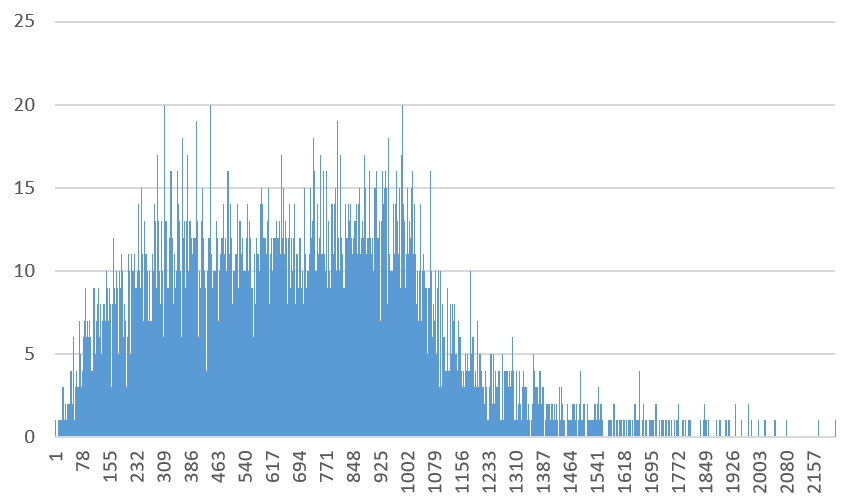
\includegraphics[width=0.7\textwidth]{figures/images/numberGenerator/overlapped.png}\label{fig:overlappedDistExample}
\end{figure}

Figure~\ref{fig:overlappedDistExample} looks completely different from figure~\ref{fig:mixedDistExample}.
No value is generated more than 20 times as opposed to the maximum amount of 350 for the mixed distribution.
In this figure no distribution is clearly visible.

The used distributions were \textasciitilde$U(1,49999)$, \textasciitilde$B(10000,0.1)$, \textasciitilde$Geo(0.001)$, powerlaw distribution with $\beta=-1.25$.
\subsection{RLS Comparison}
The following table lists the results for the RLS for inputs that are chosen from a powerlaw distribution with $\beta=-2.75$.


\makebox[\linewidth]{
\begin{tabular}{lp{3cm}p{6cm}p{6cm}}
\begin{tabular}[h]{cccccccc}
algo type&            \RLSN&     \RLSR&     \RLSR&     \RLSN&     \RLSR&     \RLSN&       RLS\\
algo param&             b=2&       s=3&       s=4&       b=3&       s=2&       b=4&         -\\
avg mut/change&       2.000&     1.996&     2.476&     3.000&     1.502&     4.000&     1.000\\
avg mut/step&         2.000&     2.000&     2.500&     3.000&     1.500&     4.000&     1.000\\
\hline
total avg count&     83,118&   104,748&   105,513&   112,223&   114,486&   121,927& 2,443,567\\
avg eval count&      83,118&   104,748&   105,513&   112,223&   114,486&   121,927&    45,834\\
max eval count&     778,110& 1,453,252&   898,974& 1,377,471&   915,268&   816,633&   485,275\\
min eval count&         197&       126&        45&       212&       271&       155&       128\\
\hline
fail ratio&           0.000&     0.000&     0.000&     0.000&     0.000&     0.000&     0.447\\
avg fail dif&             -&         -&         -&         -&         -&         -&         1\\
\end{tabular}
\end{tabular}
}


For these inputs the variants of the RLS perform differently to the binomial input.
The only similarity is the RLS being the worst as the RLS is the only algorithm that did not find an optimal solution for every input.
If the RLS did find an optimal solution in those 5 cases it would instead be the best RLS variant.
The other algorithms are ranked by the probability of flipping only one bit.
This means at first the three RLS-R variants from 2 to 3 to 4 and then the same for the RLS-N variants.
So it does seem like moving mostly one element at once is better for the geometric input in comparison to two elements for the binomial distribution.
In the 5 cases where the RLS did not find an optimal solution it was most likely stuck in a local optimum.

\subsection{(1+1) EA Comparison}
The first table again shows the results for parameter $\beta=-2.75$

\makebox[\linewidth]{
\begin{tabular}{lp{3cm}p{6cm}p{6cm}}
\begin{tabular}[h]{ccccccccc}
algo type&          (1+1) EA&   (1+1) EA&   (1+1) EA&   (1+1) EA&      (1+1) EA&   (1+1) EA&   (1+1) EA&   (1+1) EA\\
algo param&           3/n&     4/n&     2/n&     5/n&       -&    10/n&    50/n&   100/n\\
avg mut/change&     3.101&   3.968&   2.343&   4.859&   1.698&   9.732&  49.544&  99.494\\
avg mut/step&       2.999&   4.003&   2.002&   4.999&   1.001&   9.998&  49.998&  99.997\\
\hline
total avg count&      646&     701&     706&     857&   1,123&   1,508&   8,175&  15,485\\
avg eval count&       646&     701&     706&     857&   1,123&   1,508&   8,175&  15,485\\
max eval count&     5,346&   5,692&   3,415&   5,572&   7,001&  12,112&  52,831& 145,269\\
min eval count&        23&       4&      30&       9&      23&      14&      27&      69\\
\hline
fails&                  0&       0&       0&       0&       0&       0&       0&       0\\
fail ratio&         0.000&   0.000&   0.000&   0.000&   0.000&   0.000&   0.000&   0.000\\
avg fail dif&           -&       -&       -&       -&       -&       -&       -&       -\\
\end{tabular}
\end{tabular}
}


For the EA the result is also the inversion of the results for the OneMax equivalent.
The higher the mutation rate the better at least up to $n\le100$.
From mutation rate $p_m\le3/n$ the algorithm reaches the worst case at least once in 1000 runs.
If the algorithm did not manage to find an optimal solution the fitness was always the same.
So there was no run where any algorithm neither found a global nor the local optimum.
\subsection{pmut Comparison}
The first table again shows the results for parameter $\beta=-2.75$

\makebox[\linewidth]{
\scriptsize
\begin{tabular}{lp{3cm}p{6cm}p{6cm}}
\begin{tabular}[h]{m{2.5cm}m{0,40cm}m{0,40cm}m{0,40cm}m{0,40cm}m{0,40cm}m{0,40cm}m{0,40cm}m{0,40cm}m{0,40cm}m{0,40cm}m{0,40cm}m{0,40cm}m{0,40cm}m{0,40cm}m{0,40cm}m{0,40cm}m{0,40cm}m{0,40cm}}
\multicolumn{1}{c}{algo type}&\multicolumn{2}{c}{            pmut}&\multicolumn{2}{c}{     pmut}&\multicolumn{2}{c}{     pmut}&\multicolumn{2}{c}{     pmut}&\multicolumn{2}{c}{     pmut}&\multicolumn{2}{c}{     pmut}&\multicolumn{2}{c}{     pmut}&\multicolumn{2}{c}{     pmut}&\multicolumn{2}{c}{     pmut}\\
\multicolumn{1}{c}{algo param}&\multicolumn{2}{c}{           3.25}&\multicolumn{2}{c}{     3.00}&\multicolumn{2}{c}{     2.75}&\multicolumn{2}{c}{     2.50}&\multicolumn{2}{c}{     2.25}&\multicolumn{2}{c}{     2.00}&\multicolumn{2}{c}{     1.75}&\multicolumn{2}{c}{     1.50}&\multicolumn{2}{c}{     1.25}\\
\multicolumn{1}{c}{avg mut/change}&\multicolumn{2}{c}{      1.583}&\multicolumn{2}{c}{    1.737}&\multicolumn{2}{c}{    2.002}&\multicolumn{2}{c}{    2.423}&\multicolumn{2}{c}{    3.303}&\multicolumn{2}{c}{    5.830}&\multicolumn{2}{c}{   12.519}&\multicolumn{2}{c}{   30.910}&\multicolumn{2}{c}{   73.182}\\
\multicolumn{1}{c}{avg mut/step}&\multicolumn{2}{c}{        1.729}&\multicolumn{2}{c}{    1.934}&\multicolumn{2}{c}{    2.274}&\multicolumn{2}{c}{    2.895}&\multicolumn{2}{c}{    4.360}&\multicolumn{2}{c}{    8.452}&\multicolumn{2}{c}{   22.278}&\multicolumn{2}{c}{   70.532}&\multicolumn{2}{c}{  224.421}\\
\hline
\multicolumn{1}{c}{avg eval count}&\multicolumn{2}{c}{        540}&\multicolumn{2}{c}{      569}&\multicolumn{2}{c}{      594}&\multicolumn{2}{c}{      641}&\multicolumn{2}{c}{      712}&\multicolumn{2}{c}{      808}&\multicolumn{2}{c}{      967}&\multicolumn{2}{c}{    1,285}&\multicolumn{2}{c}{    2,081}\\
\multicolumn{1}{c}{max eval count}&\multicolumn{2}{c}{      3,110}&\multicolumn{2}{c}{    2,891}&\multicolumn{2}{c}{    3,504}&\multicolumn{2}{c}{    3,896}&\multicolumn{2}{c}{    5,152}&\multicolumn{2}{c}{    4,274}&\multicolumn{2}{c}{    5,610}&\multicolumn{2}{c}{    6,190}&\multicolumn{2}{c}{   14,984}\\
\multicolumn{1}{c}{min eval count}&\multicolumn{2}{c}{         22}&\multicolumn{2}{c}{        9}&\multicolumn{2}{c}{       36}&\multicolumn{2}{c}{       25}&\multicolumn{2}{c}{       28}&\multicolumn{2}{c}{       27}&\multicolumn{2}{c}{       27}&\multicolumn{2}{c}{       13}&\multicolumn{2}{c}{       33}\\
\hline
\multicolumn{1}{c}{fail ratio}&\multicolumn{2}{c}{          0.000}&\multicolumn{2}{c}{    0.000}&\multicolumn{2}{c}{    0.000}&\multicolumn{2}{c}{    0.000}&\multicolumn{2}{c}{    0.000}&\multicolumn{2}{c}{    0.000}&\multicolumn{2}{c}{    0.000}&\multicolumn{2}{c}{    0.000}&\multicolumn{2}{c}{    0.000}\\
\hline
\multicolumn{1}{c}{p-value}&&\multicolumn{2}{c}{0.0000}&\multicolumn{2}{c}{0.0000}&\multicolumn{2}{c}{0.0000}&\multicolumn{2}{c}{0.0000}&\multicolumn{2}{c}{0.0000}&\multicolumn{2}{c}{0.0000}&\multicolumn{2}{c}{0.0000}&\multicolumn{2}{c}{0.0000}\\
&&&&&&&&&&&&&&&&&&\end{tabular}
\end{tabular}
}


The ideal value for $\beta$ seems to be around -1.75 as the runtime increases for the two neighbour values.
Even the worst value still manages find an optimal solution within double the time of the best value.
The importance of the parameter is therefore not as important as for other inputs.
\subsection{Comparison of the best variants}
The first table again shows the results for parameter $\beta=-2.75$

\makebox[\linewidth]{
\begin{tabular}{lp{3cm}p{6cm}p{6cm}}
\begin{tabular}[h]{cccc}
algo type&            RLS&    pmut&      EA\\
algo param&             -&    3.25&       -\\
avg mut/change&     1.000&   1.287&   1.272\\
avg mut/step&       1.000&   1.729&   1.000\\
\hline
avg eval count&    91,171& 143,121& 231,082\\
max eval count&   153,143& 227,737& 446,942\\
min eval count&    65,783&  93,602& 165,818\\
\hline
fail ratio&         0.000&   0.000&   0.000\\
\end{tabular}
\end{tabular}
}


The results for this experiment are as expected.
All three algorithms find the optimal value within the time limit.
The RLS performs better than the (1+1) EA because it does only single bit flips.
The $pmut_{-3.25}$ perform better than the standard (1+1) EA although flipping more bits on average.
This is most likely cause by the few steps where $pmut$ flips many bits which increase the average.
But $pmut$ most likely chooses to flip only one bit more often as the (1+1) EA.

TODO insert comparison with multiple values of n.
\section{powerlaw distributed inputs}
This input is similar to the mixed input from the last subsection.
For this distribution the values are not chosen uniform random from one of the base distributions, but instead a value from every distribution is chosen and added together.
Hence the name overlapped distribution.
For this input the step limit was increased to $100\cdot n \ln n$.
The comparison with the step limit $10\cdot n \ln(n)$ is contained in the last subsubsection which compares the best variants.

\begin{figure}[h]
      \caption{Distribution of an overlapped input with \textasciitilde$U(1,999)$, \textasciitilde$B(1000,0.1)$, \textasciitilde$Geo(0.01)$, powerlaw dist with $\beta=-1.25$}
      \centering
      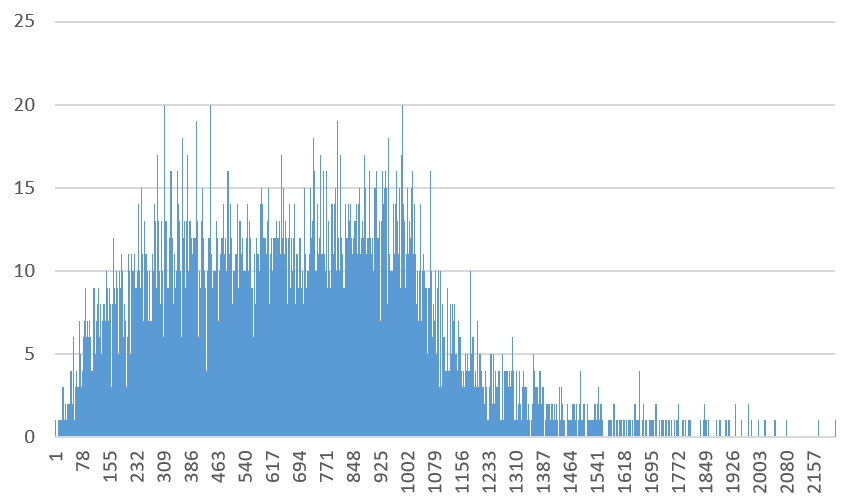
\includegraphics[width=0.7\textwidth]{figures/images/numberGenerator/overlapped.png}\label{fig:overlappedDistExample}
\end{figure}

Figure~\ref{fig:overlappedDistExample} looks completely different from figure~\ref{fig:mixedDistExample}.
No value is generated more than 20 times as opposed to the maximum amount of 350 for the mixed distribution.
In this figure no distribution is clearly visible.

The used distributions were \textasciitilde$U(1,49999)$, \textasciitilde$B(10000,0.1)$, \textasciitilde$Geo(0.001)$, powerlaw distribution with $\beta=-1.25$.
\subsection{RLS Comparison}
The following table lists the results for the RLS for inputs that are chosen from a powerlaw distribution with $\beta=-2.75$.


\makebox[\linewidth]{
\begin{tabular}{lp{3cm}p{6cm}p{6cm}}
\begin{tabular}[h]{cccccccc}
algo type&            \RLSN&     \RLSR&     \RLSR&     \RLSN&     \RLSR&     \RLSN&       RLS\\
algo param&             b=2&       s=3&       s=4&       b=3&       s=2&       b=4&         -\\
avg mut/change&       2.000&     1.996&     2.476&     3.000&     1.502&     4.000&     1.000\\
avg mut/step&         2.000&     2.000&     2.500&     3.000&     1.500&     4.000&     1.000\\
\hline
total avg count&     83,118&   104,748&   105,513&   112,223&   114,486&   121,927& 2,443,567\\
avg eval count&      83,118&   104,748&   105,513&   112,223&   114,486&   121,927&    45,834\\
max eval count&     778,110& 1,453,252&   898,974& 1,377,471&   915,268&   816,633&   485,275\\
min eval count&         197&       126&        45&       212&       271&       155&       128\\
\hline
fail ratio&           0.000&     0.000&     0.000&     0.000&     0.000&     0.000&     0.447\\
avg fail dif&             -&         -&         -&         -&         -&         -&         1\\
\end{tabular}
\end{tabular}
}


For these inputs the variants of the RLS perform differently to the binomial input.
The only similarity is the RLS being the worst as the RLS is the only algorithm that did not find an optimal solution for every input.
If the RLS did find an optimal solution in those 5 cases it would instead be the best RLS variant.
The other algorithms are ranked by the probability of flipping only one bit.
This means at first the three RLS-R variants from 2 to 3 to 4 and then the same for the RLS-N variants.
So it does seem like moving mostly one element at once is better for the geometric input in comparison to two elements for the binomial distribution.
In the 5 cases where the RLS did not find an optimal solution it was most likely stuck in a local optimum.

\subsection{(1+1) EA Comparison}
The first table again shows the results for parameter $\beta=-2.75$

\makebox[\linewidth]{
\begin{tabular}{lp{3cm}p{6cm}p{6cm}}
\begin{tabular}[h]{ccccccccc}
algo type&          (1+1) EA&   (1+1) EA&   (1+1) EA&   (1+1) EA&      (1+1) EA&   (1+1) EA&   (1+1) EA&   (1+1) EA\\
algo param&           3/n&     4/n&     2/n&     5/n&       -&    10/n&    50/n&   100/n\\
avg mut/change&     3.101&   3.968&   2.343&   4.859&   1.698&   9.732&  49.544&  99.494\\
avg mut/step&       2.999&   4.003&   2.002&   4.999&   1.001&   9.998&  49.998&  99.997\\
\hline
total avg count&      646&     701&     706&     857&   1,123&   1,508&   8,175&  15,485\\
avg eval count&       646&     701&     706&     857&   1,123&   1,508&   8,175&  15,485\\
max eval count&     5,346&   5,692&   3,415&   5,572&   7,001&  12,112&  52,831& 145,269\\
min eval count&        23&       4&      30&       9&      23&      14&      27&      69\\
\hline
fails&                  0&       0&       0&       0&       0&       0&       0&       0\\
fail ratio&         0.000&   0.000&   0.000&   0.000&   0.000&   0.000&   0.000&   0.000\\
avg fail dif&           -&       -&       -&       -&       -&       -&       -&       -\\
\end{tabular}
\end{tabular}
}


For the EA the result is also the inversion of the results for the OneMax equivalent.
The higher the mutation rate the better at least up to $n\le100$.
From mutation rate $p_m\le3/n$ the algorithm reaches the worst case at least once in 1000 runs.
If the algorithm did not manage to find an optimal solution the fitness was always the same.
So there was no run where any algorithm neither found a global nor the local optimum.
\subsection{pmut Comparison}
The first table again shows the results for parameter $\beta=-2.75$

\makebox[\linewidth]{
\scriptsize
\begin{tabular}{lp{3cm}p{6cm}p{6cm}}
\begin{tabular}[h]{m{2.5cm}m{0,40cm}m{0,40cm}m{0,40cm}m{0,40cm}m{0,40cm}m{0,40cm}m{0,40cm}m{0,40cm}m{0,40cm}m{0,40cm}m{0,40cm}m{0,40cm}m{0,40cm}m{0,40cm}m{0,40cm}m{0,40cm}m{0,40cm}m{0,40cm}}
\multicolumn{1}{c}{algo type}&\multicolumn{2}{c}{            pmut}&\multicolumn{2}{c}{     pmut}&\multicolumn{2}{c}{     pmut}&\multicolumn{2}{c}{     pmut}&\multicolumn{2}{c}{     pmut}&\multicolumn{2}{c}{     pmut}&\multicolumn{2}{c}{     pmut}&\multicolumn{2}{c}{     pmut}&\multicolumn{2}{c}{     pmut}\\
\multicolumn{1}{c}{algo param}&\multicolumn{2}{c}{           3.25}&\multicolumn{2}{c}{     3.00}&\multicolumn{2}{c}{     2.75}&\multicolumn{2}{c}{     2.50}&\multicolumn{2}{c}{     2.25}&\multicolumn{2}{c}{     2.00}&\multicolumn{2}{c}{     1.75}&\multicolumn{2}{c}{     1.50}&\multicolumn{2}{c}{     1.25}\\
\multicolumn{1}{c}{avg mut/change}&\multicolumn{2}{c}{      1.583}&\multicolumn{2}{c}{    1.737}&\multicolumn{2}{c}{    2.002}&\multicolumn{2}{c}{    2.423}&\multicolumn{2}{c}{    3.303}&\multicolumn{2}{c}{    5.830}&\multicolumn{2}{c}{   12.519}&\multicolumn{2}{c}{   30.910}&\multicolumn{2}{c}{   73.182}\\
\multicolumn{1}{c}{avg mut/step}&\multicolumn{2}{c}{        1.729}&\multicolumn{2}{c}{    1.934}&\multicolumn{2}{c}{    2.274}&\multicolumn{2}{c}{    2.895}&\multicolumn{2}{c}{    4.360}&\multicolumn{2}{c}{    8.452}&\multicolumn{2}{c}{   22.278}&\multicolumn{2}{c}{   70.532}&\multicolumn{2}{c}{  224.421}\\
\hline
\multicolumn{1}{c}{avg eval count}&\multicolumn{2}{c}{        540}&\multicolumn{2}{c}{      569}&\multicolumn{2}{c}{      594}&\multicolumn{2}{c}{      641}&\multicolumn{2}{c}{      712}&\multicolumn{2}{c}{      808}&\multicolumn{2}{c}{      967}&\multicolumn{2}{c}{    1,285}&\multicolumn{2}{c}{    2,081}\\
\multicolumn{1}{c}{max eval count}&\multicolumn{2}{c}{      3,110}&\multicolumn{2}{c}{    2,891}&\multicolumn{2}{c}{    3,504}&\multicolumn{2}{c}{    3,896}&\multicolumn{2}{c}{    5,152}&\multicolumn{2}{c}{    4,274}&\multicolumn{2}{c}{    5,610}&\multicolumn{2}{c}{    6,190}&\multicolumn{2}{c}{   14,984}\\
\multicolumn{1}{c}{min eval count}&\multicolumn{2}{c}{         22}&\multicolumn{2}{c}{        9}&\multicolumn{2}{c}{       36}&\multicolumn{2}{c}{       25}&\multicolumn{2}{c}{       28}&\multicolumn{2}{c}{       27}&\multicolumn{2}{c}{       27}&\multicolumn{2}{c}{       13}&\multicolumn{2}{c}{       33}\\
\hline
\multicolumn{1}{c}{fail ratio}&\multicolumn{2}{c}{          0.000}&\multicolumn{2}{c}{    0.000}&\multicolumn{2}{c}{    0.000}&\multicolumn{2}{c}{    0.000}&\multicolumn{2}{c}{    0.000}&\multicolumn{2}{c}{    0.000}&\multicolumn{2}{c}{    0.000}&\multicolumn{2}{c}{    0.000}&\multicolumn{2}{c}{    0.000}\\
\hline
\multicolumn{1}{c}{p-value}&&\multicolumn{2}{c}{0.0000}&\multicolumn{2}{c}{0.0000}&\multicolumn{2}{c}{0.0000}&\multicolumn{2}{c}{0.0000}&\multicolumn{2}{c}{0.0000}&\multicolumn{2}{c}{0.0000}&\multicolumn{2}{c}{0.0000}&\multicolumn{2}{c}{0.0000}\\
&&&&&&&&&&&&&&&&&&\end{tabular}
\end{tabular}
}


The ideal value for $\beta$ seems to be around -1.75 as the runtime increases for the two neighbour values.
Even the worst value still manages find an optimal solution within double the time of the best value.
The importance of the parameter is therefore not as important as for other inputs.
\subsection{Comparison of the best variants}
The first table again shows the results for parameter $\beta=-2.75$

\makebox[\linewidth]{
\begin{tabular}{lp{3cm}p{6cm}p{6cm}}
\begin{tabular}[h]{cccc}
algo type&            RLS&    pmut&      EA\\
algo param&             -&    3.25&       -\\
avg mut/change&     1.000&   1.287&   1.272\\
avg mut/step&       1.000&   1.729&   1.000\\
\hline
avg eval count&    91,171& 143,121& 231,082\\
max eval count&   153,143& 227,737& 446,942\\
min eval count&    65,783&  93,602& 165,818\\
\hline
fail ratio&         0.000&   0.000&   0.000\\
\end{tabular}
\end{tabular}
}


The results for this experiment are as expected.
All three algorithms find the optimal value within the time limit.
The RLS performs better than the (1+1) EA because it does only single bit flips.
The $pmut_{-3.25}$ perform better than the standard (1+1) EA although flipping more bits on average.
This is most likely cause by the few steps where $pmut$ flips many bits which increase the average.
But $pmut$ most likely chooses to flip only one bit more often as the (1+1) EA.

TODO insert comparison with multiple values of n.
\section{OneMax Equivalent for PARTITION}
This input is similar to the mixed input from the last subsection.
For this distribution the values are not chosen uniform random from one of the base distributions, but instead a value from every distribution is chosen and added together.
Hence the name overlapped distribution.
For this input the step limit was increased to $100\cdot n \ln n$.
The comparison with the step limit $10\cdot n \ln(n)$ is contained in the last subsubsection which compares the best variants.

\begin{figure}[h]
      \caption{Distribution of an overlapped input with \textasciitilde$U(1,999)$, \textasciitilde$B(1000,0.1)$, \textasciitilde$Geo(0.01)$, powerlaw dist with $\beta=-1.25$}
      \centering
      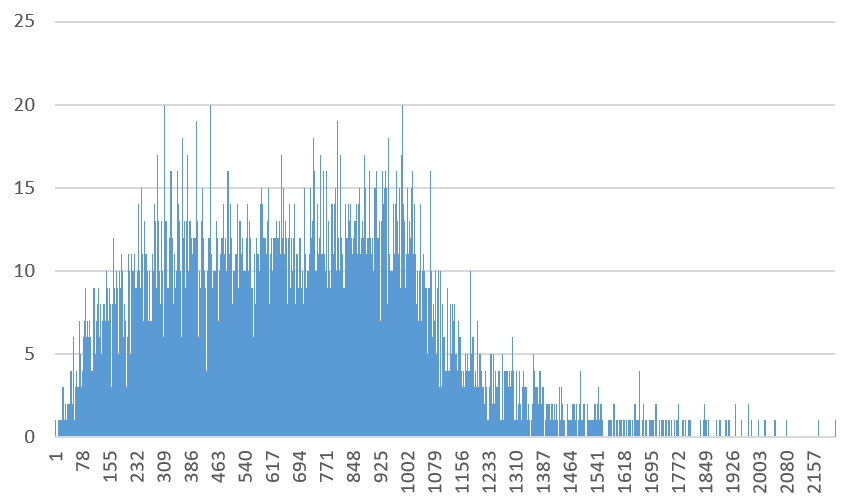
\includegraphics[width=0.7\textwidth]{figures/images/numberGenerator/overlapped.png}\label{fig:overlappedDistExample}
\end{figure}

Figure~\ref{fig:overlappedDistExample} looks completely different from figure~\ref{fig:mixedDistExample}.
No value is generated more than 20 times as opposed to the maximum amount of 350 for the mixed distribution.
In this figure no distribution is clearly visible.

The used distributions were \textasciitilde$U(1,49999)$, \textasciitilde$B(10000,0.1)$, \textasciitilde$Geo(0.001)$, powerlaw distribution with $\beta=-1.25$.
\subsection{RLS Comparison}
The following table lists the results for the RLS for inputs that are chosen from a powerlaw distribution with $\beta=-2.75$.


\makebox[\linewidth]{
\begin{tabular}{lp{3cm}p{6cm}p{6cm}}
\begin{tabular}[h]{cccccccc}
algo type&            \RLSN&     \RLSR&     \RLSR&     \RLSN&     \RLSR&     \RLSN&       RLS\\
algo param&             b=2&       s=3&       s=4&       b=3&       s=2&       b=4&         -\\
avg mut/change&       2.000&     1.996&     2.476&     3.000&     1.502&     4.000&     1.000\\
avg mut/step&         2.000&     2.000&     2.500&     3.000&     1.500&     4.000&     1.000\\
\hline
total avg count&     83,118&   104,748&   105,513&   112,223&   114,486&   121,927& 2,443,567\\
avg eval count&      83,118&   104,748&   105,513&   112,223&   114,486&   121,927&    45,834\\
max eval count&     778,110& 1,453,252&   898,974& 1,377,471&   915,268&   816,633&   485,275\\
min eval count&         197&       126&        45&       212&       271&       155&       128\\
\hline
fail ratio&           0.000&     0.000&     0.000&     0.000&     0.000&     0.000&     0.447\\
avg fail dif&             -&         -&         -&         -&         -&         -&         1\\
\end{tabular}
\end{tabular}
}


For these inputs the variants of the RLS perform differently to the binomial input.
The only similarity is the RLS being the worst as the RLS is the only algorithm that did not find an optimal solution for every input.
If the RLS did find an optimal solution in those 5 cases it would instead be the best RLS variant.
The other algorithms are ranked by the probability of flipping only one bit.
This means at first the three RLS-R variants from 2 to 3 to 4 and then the same for the RLS-N variants.
So it does seem like moving mostly one element at once is better for the geometric input in comparison to two elements for the binomial distribution.
In the 5 cases where the RLS did not find an optimal solution it was most likely stuck in a local optimum.

\subsection{(1+1) EA Comparison}
The first table again shows the results for parameter $\beta=-2.75$

\makebox[\linewidth]{
\begin{tabular}{lp{3cm}p{6cm}p{6cm}}
\begin{tabular}[h]{ccccccccc}
algo type&          (1+1) EA&   (1+1) EA&   (1+1) EA&   (1+1) EA&      (1+1) EA&   (1+1) EA&   (1+1) EA&   (1+1) EA\\
algo param&           3/n&     4/n&     2/n&     5/n&       -&    10/n&    50/n&   100/n\\
avg mut/change&     3.101&   3.968&   2.343&   4.859&   1.698&   9.732&  49.544&  99.494\\
avg mut/step&       2.999&   4.003&   2.002&   4.999&   1.001&   9.998&  49.998&  99.997\\
\hline
total avg count&      646&     701&     706&     857&   1,123&   1,508&   8,175&  15,485\\
avg eval count&       646&     701&     706&     857&   1,123&   1,508&   8,175&  15,485\\
max eval count&     5,346&   5,692&   3,415&   5,572&   7,001&  12,112&  52,831& 145,269\\
min eval count&        23&       4&      30&       9&      23&      14&      27&      69\\
\hline
fails&                  0&       0&       0&       0&       0&       0&       0&       0\\
fail ratio&         0.000&   0.000&   0.000&   0.000&   0.000&   0.000&   0.000&   0.000\\
avg fail dif&           -&       -&       -&       -&       -&       -&       -&       -\\
\end{tabular}
\end{tabular}
}


For the EA the result is also the inversion of the results for the OneMax equivalent.
The higher the mutation rate the better at least up to $n\le100$.
From mutation rate $p_m\le3/n$ the algorithm reaches the worst case at least once in 1000 runs.
If the algorithm did not manage to find an optimal solution the fitness was always the same.
So there was no run where any algorithm neither found a global nor the local optimum.
\subsection{pmut Comparison}
The first table again shows the results for parameter $\beta=-2.75$

\makebox[\linewidth]{
\scriptsize
\begin{tabular}{lp{3cm}p{6cm}p{6cm}}
\begin{tabular}[h]{m{2.5cm}m{0,40cm}m{0,40cm}m{0,40cm}m{0,40cm}m{0,40cm}m{0,40cm}m{0,40cm}m{0,40cm}m{0,40cm}m{0,40cm}m{0,40cm}m{0,40cm}m{0,40cm}m{0,40cm}m{0,40cm}m{0,40cm}m{0,40cm}m{0,40cm}}
\multicolumn{1}{c}{algo type}&\multicolumn{2}{c}{            pmut}&\multicolumn{2}{c}{     pmut}&\multicolumn{2}{c}{     pmut}&\multicolumn{2}{c}{     pmut}&\multicolumn{2}{c}{     pmut}&\multicolumn{2}{c}{     pmut}&\multicolumn{2}{c}{     pmut}&\multicolumn{2}{c}{     pmut}&\multicolumn{2}{c}{     pmut}\\
\multicolumn{1}{c}{algo param}&\multicolumn{2}{c}{           3.25}&\multicolumn{2}{c}{     3.00}&\multicolumn{2}{c}{     2.75}&\multicolumn{2}{c}{     2.50}&\multicolumn{2}{c}{     2.25}&\multicolumn{2}{c}{     2.00}&\multicolumn{2}{c}{     1.75}&\multicolumn{2}{c}{     1.50}&\multicolumn{2}{c}{     1.25}\\
\multicolumn{1}{c}{avg mut/change}&\multicolumn{2}{c}{      1.583}&\multicolumn{2}{c}{    1.737}&\multicolumn{2}{c}{    2.002}&\multicolumn{2}{c}{    2.423}&\multicolumn{2}{c}{    3.303}&\multicolumn{2}{c}{    5.830}&\multicolumn{2}{c}{   12.519}&\multicolumn{2}{c}{   30.910}&\multicolumn{2}{c}{   73.182}\\
\multicolumn{1}{c}{avg mut/step}&\multicolumn{2}{c}{        1.729}&\multicolumn{2}{c}{    1.934}&\multicolumn{2}{c}{    2.274}&\multicolumn{2}{c}{    2.895}&\multicolumn{2}{c}{    4.360}&\multicolumn{2}{c}{    8.452}&\multicolumn{2}{c}{   22.278}&\multicolumn{2}{c}{   70.532}&\multicolumn{2}{c}{  224.421}\\
\hline
\multicolumn{1}{c}{avg eval count}&\multicolumn{2}{c}{        540}&\multicolumn{2}{c}{      569}&\multicolumn{2}{c}{      594}&\multicolumn{2}{c}{      641}&\multicolumn{2}{c}{      712}&\multicolumn{2}{c}{      808}&\multicolumn{2}{c}{      967}&\multicolumn{2}{c}{    1,285}&\multicolumn{2}{c}{    2,081}\\
\multicolumn{1}{c}{max eval count}&\multicolumn{2}{c}{      3,110}&\multicolumn{2}{c}{    2,891}&\multicolumn{2}{c}{    3,504}&\multicolumn{2}{c}{    3,896}&\multicolumn{2}{c}{    5,152}&\multicolumn{2}{c}{    4,274}&\multicolumn{2}{c}{    5,610}&\multicolumn{2}{c}{    6,190}&\multicolumn{2}{c}{   14,984}\\
\multicolumn{1}{c}{min eval count}&\multicolumn{2}{c}{         22}&\multicolumn{2}{c}{        9}&\multicolumn{2}{c}{       36}&\multicolumn{2}{c}{       25}&\multicolumn{2}{c}{       28}&\multicolumn{2}{c}{       27}&\multicolumn{2}{c}{       27}&\multicolumn{2}{c}{       13}&\multicolumn{2}{c}{       33}\\
\hline
\multicolumn{1}{c}{fail ratio}&\multicolumn{2}{c}{          0.000}&\multicolumn{2}{c}{    0.000}&\multicolumn{2}{c}{    0.000}&\multicolumn{2}{c}{    0.000}&\multicolumn{2}{c}{    0.000}&\multicolumn{2}{c}{    0.000}&\multicolumn{2}{c}{    0.000}&\multicolumn{2}{c}{    0.000}&\multicolumn{2}{c}{    0.000}\\
\hline
\multicolumn{1}{c}{p-value}&&\multicolumn{2}{c}{0.0000}&\multicolumn{2}{c}{0.0000}&\multicolumn{2}{c}{0.0000}&\multicolumn{2}{c}{0.0000}&\multicolumn{2}{c}{0.0000}&\multicolumn{2}{c}{0.0000}&\multicolumn{2}{c}{0.0000}&\multicolumn{2}{c}{0.0000}\\
&&&&&&&&&&&&&&&&&&\end{tabular}
\end{tabular}
}


The ideal value for $\beta$ seems to be around -1.75 as the runtime increases for the two neighbour values.
Even the worst value still manages find an optimal solution within double the time of the best value.
The importance of the parameter is therefore not as important as for other inputs.
\subsection{Comparison of the best variants}
The first table again shows the results for parameter $\beta=-2.75$

\makebox[\linewidth]{
\begin{tabular}{lp{3cm}p{6cm}p{6cm}}
\begin{tabular}[h]{cccc}
algo type&            RLS&    pmut&      EA\\
algo param&             -&    3.25&       -\\
avg mut/change&     1.000&   1.287&   1.272\\
avg mut/step&       1.000&   1.729&   1.000\\
\hline
avg eval count&    91,171& 143,121& 231,082\\
max eval count&   153,143& 227,737& 446,942\\
min eval count&    65,783&  93,602& 165,818\\
\hline
fail ratio&         0.000&   0.000&   0.000\\
\end{tabular}
\end{tabular}
}


The results for this experiment are as expected.
All three algorithms find the optimal value within the time limit.
The RLS performs better than the (1+1) EA because it does only single bit flips.
The $pmut_{-3.25}$ perform better than the standard (1+1) EA although flipping more bits on average.
This is most likely cause by the few steps where $pmut$ flips many bits which increase the average.
But $pmut$ most likely chooses to flip only one bit more often as the (1+1) EA.

TODO insert comparison with multiple values of n.
\section{Carsten Witts worst case input}
This input is similar to the mixed input from the last subsection.
For this distribution the values are not chosen uniform random from one of the base distributions, but instead a value from every distribution is chosen and added together.
Hence the name overlapped distribution.
For this input the step limit was increased to $100\cdot n \ln n$.
The comparison with the step limit $10\cdot n \ln(n)$ is contained in the last subsubsection which compares the best variants.

\begin{figure}[h]
      \caption{Distribution of an overlapped input with \textasciitilde$U(1,999)$, \textasciitilde$B(1000,0.1)$, \textasciitilde$Geo(0.01)$, powerlaw dist with $\beta=-1.25$}
      \centering
      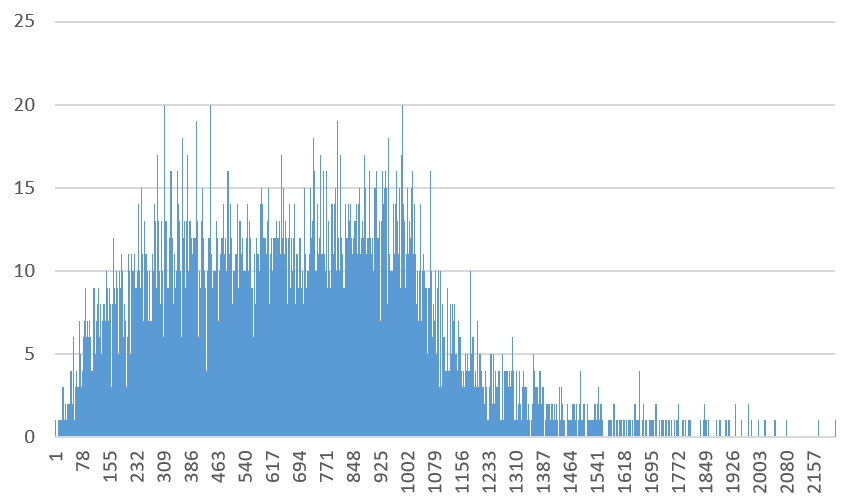
\includegraphics[width=0.7\textwidth]{figures/images/numberGenerator/overlapped.png}\label{fig:overlappedDistExample}
\end{figure}

Figure~\ref{fig:overlappedDistExample} looks completely different from figure~\ref{fig:mixedDistExample}.
No value is generated more than 20 times as opposed to the maximum amount of 350 for the mixed distribution.
In this figure no distribution is clearly visible.

The used distributions were \textasciitilde$U(1,49999)$, \textasciitilde$B(10000,0.1)$, \textasciitilde$Geo(0.001)$, powerlaw distribution with $\beta=-1.25$.
\subsection{RLS Comparison}
The following table lists the results for the RLS for inputs that are chosen from a powerlaw distribution with $\beta=-2.75$.


\makebox[\linewidth]{
\begin{tabular}{lp{3cm}p{6cm}p{6cm}}
\begin{tabular}[h]{cccccccc}
algo type&            \RLSN&     \RLSR&     \RLSR&     \RLSN&     \RLSR&     \RLSN&       RLS\\
algo param&             b=2&       s=3&       s=4&       b=3&       s=2&       b=4&         -\\
avg mut/change&       2.000&     1.996&     2.476&     3.000&     1.502&     4.000&     1.000\\
avg mut/step&         2.000&     2.000&     2.500&     3.000&     1.500&     4.000&     1.000\\
\hline
total avg count&     83,118&   104,748&   105,513&   112,223&   114,486&   121,927& 2,443,567\\
avg eval count&      83,118&   104,748&   105,513&   112,223&   114,486&   121,927&    45,834\\
max eval count&     778,110& 1,453,252&   898,974& 1,377,471&   915,268&   816,633&   485,275\\
min eval count&         197&       126&        45&       212&       271&       155&       128\\
\hline
fail ratio&           0.000&     0.000&     0.000&     0.000&     0.000&     0.000&     0.447\\
avg fail dif&             -&         -&         -&         -&         -&         -&         1\\
\end{tabular}
\end{tabular}
}


For these inputs the variants of the RLS perform differently to the binomial input.
The only similarity is the RLS being the worst as the RLS is the only algorithm that did not find an optimal solution for every input.
If the RLS did find an optimal solution in those 5 cases it would instead be the best RLS variant.
The other algorithms are ranked by the probability of flipping only one bit.
This means at first the three RLS-R variants from 2 to 3 to 4 and then the same for the RLS-N variants.
So it does seem like moving mostly one element at once is better for the geometric input in comparison to two elements for the binomial distribution.
In the 5 cases where the RLS did not find an optimal solution it was most likely stuck in a local optimum.

\subsection{(1+1) EA Comparison}
The first table again shows the results for parameter $\beta=-2.75$

\makebox[\linewidth]{
\begin{tabular}{lp{3cm}p{6cm}p{6cm}}
\begin{tabular}[h]{ccccccccc}
algo type&          (1+1) EA&   (1+1) EA&   (1+1) EA&   (1+1) EA&      (1+1) EA&   (1+1) EA&   (1+1) EA&   (1+1) EA\\
algo param&           3/n&     4/n&     2/n&     5/n&       -&    10/n&    50/n&   100/n\\
avg mut/change&     3.101&   3.968&   2.343&   4.859&   1.698&   9.732&  49.544&  99.494\\
avg mut/step&       2.999&   4.003&   2.002&   4.999&   1.001&   9.998&  49.998&  99.997\\
\hline
total avg count&      646&     701&     706&     857&   1,123&   1,508&   8,175&  15,485\\
avg eval count&       646&     701&     706&     857&   1,123&   1,508&   8,175&  15,485\\
max eval count&     5,346&   5,692&   3,415&   5,572&   7,001&  12,112&  52,831& 145,269\\
min eval count&        23&       4&      30&       9&      23&      14&      27&      69\\
\hline
fails&                  0&       0&       0&       0&       0&       0&       0&       0\\
fail ratio&         0.000&   0.000&   0.000&   0.000&   0.000&   0.000&   0.000&   0.000\\
avg fail dif&           -&       -&       -&       -&       -&       -&       -&       -\\
\end{tabular}
\end{tabular}
}


For the EA the result is also the inversion of the results for the OneMax equivalent.
The higher the mutation rate the better at least up to $n\le100$.
From mutation rate $p_m\le3/n$ the algorithm reaches the worst case at least once in 1000 runs.
If the algorithm did not manage to find an optimal solution the fitness was always the same.
So there was no run where any algorithm neither found a global nor the local optimum.
\subsection{pmut Comparison}
The first table again shows the results for parameter $\beta=-2.75$

\makebox[\linewidth]{
\scriptsize
\begin{tabular}{lp{3cm}p{6cm}p{6cm}}
\begin{tabular}[h]{m{2.5cm}m{0,40cm}m{0,40cm}m{0,40cm}m{0,40cm}m{0,40cm}m{0,40cm}m{0,40cm}m{0,40cm}m{0,40cm}m{0,40cm}m{0,40cm}m{0,40cm}m{0,40cm}m{0,40cm}m{0,40cm}m{0,40cm}m{0,40cm}m{0,40cm}}
\multicolumn{1}{c}{algo type}&\multicolumn{2}{c}{            pmut}&\multicolumn{2}{c}{     pmut}&\multicolumn{2}{c}{     pmut}&\multicolumn{2}{c}{     pmut}&\multicolumn{2}{c}{     pmut}&\multicolumn{2}{c}{     pmut}&\multicolumn{2}{c}{     pmut}&\multicolumn{2}{c}{     pmut}&\multicolumn{2}{c}{     pmut}\\
\multicolumn{1}{c}{algo param}&\multicolumn{2}{c}{           3.25}&\multicolumn{2}{c}{     3.00}&\multicolumn{2}{c}{     2.75}&\multicolumn{2}{c}{     2.50}&\multicolumn{2}{c}{     2.25}&\multicolumn{2}{c}{     2.00}&\multicolumn{2}{c}{     1.75}&\multicolumn{2}{c}{     1.50}&\multicolumn{2}{c}{     1.25}\\
\multicolumn{1}{c}{avg mut/change}&\multicolumn{2}{c}{      1.583}&\multicolumn{2}{c}{    1.737}&\multicolumn{2}{c}{    2.002}&\multicolumn{2}{c}{    2.423}&\multicolumn{2}{c}{    3.303}&\multicolumn{2}{c}{    5.830}&\multicolumn{2}{c}{   12.519}&\multicolumn{2}{c}{   30.910}&\multicolumn{2}{c}{   73.182}\\
\multicolumn{1}{c}{avg mut/step}&\multicolumn{2}{c}{        1.729}&\multicolumn{2}{c}{    1.934}&\multicolumn{2}{c}{    2.274}&\multicolumn{2}{c}{    2.895}&\multicolumn{2}{c}{    4.360}&\multicolumn{2}{c}{    8.452}&\multicolumn{2}{c}{   22.278}&\multicolumn{2}{c}{   70.532}&\multicolumn{2}{c}{  224.421}\\
\hline
\multicolumn{1}{c}{avg eval count}&\multicolumn{2}{c}{        540}&\multicolumn{2}{c}{      569}&\multicolumn{2}{c}{      594}&\multicolumn{2}{c}{      641}&\multicolumn{2}{c}{      712}&\multicolumn{2}{c}{      808}&\multicolumn{2}{c}{      967}&\multicolumn{2}{c}{    1,285}&\multicolumn{2}{c}{    2,081}\\
\multicolumn{1}{c}{max eval count}&\multicolumn{2}{c}{      3,110}&\multicolumn{2}{c}{    2,891}&\multicolumn{2}{c}{    3,504}&\multicolumn{2}{c}{    3,896}&\multicolumn{2}{c}{    5,152}&\multicolumn{2}{c}{    4,274}&\multicolumn{2}{c}{    5,610}&\multicolumn{2}{c}{    6,190}&\multicolumn{2}{c}{   14,984}\\
\multicolumn{1}{c}{min eval count}&\multicolumn{2}{c}{         22}&\multicolumn{2}{c}{        9}&\multicolumn{2}{c}{       36}&\multicolumn{2}{c}{       25}&\multicolumn{2}{c}{       28}&\multicolumn{2}{c}{       27}&\multicolumn{2}{c}{       27}&\multicolumn{2}{c}{       13}&\multicolumn{2}{c}{       33}\\
\hline
\multicolumn{1}{c}{fail ratio}&\multicolumn{2}{c}{          0.000}&\multicolumn{2}{c}{    0.000}&\multicolumn{2}{c}{    0.000}&\multicolumn{2}{c}{    0.000}&\multicolumn{2}{c}{    0.000}&\multicolumn{2}{c}{    0.000}&\multicolumn{2}{c}{    0.000}&\multicolumn{2}{c}{    0.000}&\multicolumn{2}{c}{    0.000}\\
\hline
\multicolumn{1}{c}{p-value}&&\multicolumn{2}{c}{0.0000}&\multicolumn{2}{c}{0.0000}&\multicolumn{2}{c}{0.0000}&\multicolumn{2}{c}{0.0000}&\multicolumn{2}{c}{0.0000}&\multicolumn{2}{c}{0.0000}&\multicolumn{2}{c}{0.0000}&\multicolumn{2}{c}{0.0000}\\
&&&&&&&&&&&&&&&&&&\end{tabular}
\end{tabular}
}


The ideal value for $\beta$ seems to be around -1.75 as the runtime increases for the two neighbour values.
Even the worst value still manages find an optimal solution within double the time of the best value.
The importance of the parameter is therefore not as important as for other inputs.
\subsection{Comparison of the best variants}
The first table again shows the results for parameter $\beta=-2.75$

\makebox[\linewidth]{
\begin{tabular}{lp{3cm}p{6cm}p{6cm}}
\begin{tabular}[h]{cccc}
algo type&            RLS&    pmut&      EA\\
algo param&             -&    3.25&       -\\
avg mut/change&     1.000&   1.287&   1.272\\
avg mut/step&       1.000&   1.729&   1.000\\
\hline
avg eval count&    91,171& 143,121& 231,082\\
max eval count&   153,143& 227,737& 446,942\\
min eval count&    65,783&  93,602& 165,818\\
\hline
fail ratio&         0.000&   0.000&   0.000\\
\end{tabular}
\end{tabular}
}


The results for this experiment are as expected.
All three algorithms find the optimal value within the time limit.
The RLS performs better than the (1+1) EA because it does only single bit flips.
The $pmut_{-3.25}$ perform better than the standard (1+1) EA although flipping more bits on average.
This is most likely cause by the few steps where $pmut$ flips many bits which increase the average.
But $pmut$ most likely chooses to flip only one bit more often as the (1+1) EA.

TODO insert comparison with multiple values of n.
\section{Multiple distributions mixed}
This input is similar to the mixed input from the last subsection.
For this distribution the values are not chosen uniform random from one of the base distributions, but instead a value from every distribution is chosen and added together.
Hence the name overlapped distribution.
For this input the step limit was increased to $100\cdot n \ln n$.
The comparison with the step limit $10\cdot n \ln(n)$ is contained in the last subsubsection which compares the best variants.

\begin{figure}[h]
      \caption{Distribution of an overlapped input with \textasciitilde$U(1,999)$, \textasciitilde$B(1000,0.1)$, \textasciitilde$Geo(0.01)$, powerlaw dist with $\beta=-1.25$}
      \centering
      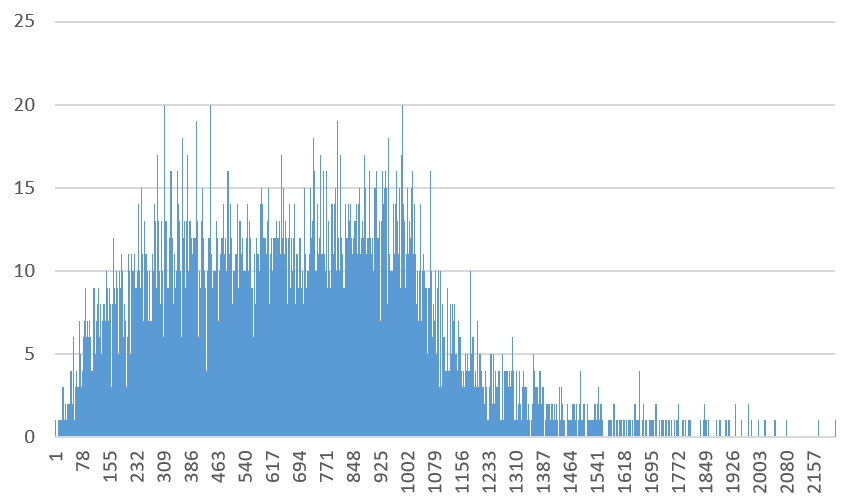
\includegraphics[width=0.7\textwidth]{figures/images/numberGenerator/overlapped.png}\label{fig:overlappedDistExample}
\end{figure}

Figure~\ref{fig:overlappedDistExample} looks completely different from figure~\ref{fig:mixedDistExample}.
No value is generated more than 20 times as opposed to the maximum amount of 350 for the mixed distribution.
In this figure no distribution is clearly visible.

The used distributions were \textasciitilde$U(1,49999)$, \textasciitilde$B(10000,0.1)$, \textasciitilde$Geo(0.001)$, powerlaw distribution with $\beta=-1.25$.
\subsection{RLS Comparison}
The following table lists the results for the RLS for inputs that are chosen from a powerlaw distribution with $\beta=-2.75$.


\makebox[\linewidth]{
\begin{tabular}{lp{3cm}p{6cm}p{6cm}}
\begin{tabular}[h]{cccccccc}
algo type&            \RLSN&     \RLSR&     \RLSR&     \RLSN&     \RLSR&     \RLSN&       RLS\\
algo param&             b=2&       s=3&       s=4&       b=3&       s=2&       b=4&         -\\
avg mut/change&       2.000&     1.996&     2.476&     3.000&     1.502&     4.000&     1.000\\
avg mut/step&         2.000&     2.000&     2.500&     3.000&     1.500&     4.000&     1.000\\
\hline
total avg count&     83,118&   104,748&   105,513&   112,223&   114,486&   121,927& 2,443,567\\
avg eval count&      83,118&   104,748&   105,513&   112,223&   114,486&   121,927&    45,834\\
max eval count&     778,110& 1,453,252&   898,974& 1,377,471&   915,268&   816,633&   485,275\\
min eval count&         197&       126&        45&       212&       271&       155&       128\\
\hline
fail ratio&           0.000&     0.000&     0.000&     0.000&     0.000&     0.000&     0.447\\
avg fail dif&             -&         -&         -&         -&         -&         -&         1\\
\end{tabular}
\end{tabular}
}


For these inputs the variants of the RLS perform differently to the binomial input.
The only similarity is the RLS being the worst as the RLS is the only algorithm that did not find an optimal solution for every input.
If the RLS did find an optimal solution in those 5 cases it would instead be the best RLS variant.
The other algorithms are ranked by the probability of flipping only one bit.
This means at first the three RLS-R variants from 2 to 3 to 4 and then the same for the RLS-N variants.
So it does seem like moving mostly one element at once is better for the geometric input in comparison to two elements for the binomial distribution.
In the 5 cases where the RLS did not find an optimal solution it was most likely stuck in a local optimum.

\subsection{(1+1) EA Comparison}
The first table again shows the results for parameter $\beta=-2.75$

\makebox[\linewidth]{
\begin{tabular}{lp{3cm}p{6cm}p{6cm}}
\begin{tabular}[h]{ccccccccc}
algo type&          (1+1) EA&   (1+1) EA&   (1+1) EA&   (1+1) EA&      (1+1) EA&   (1+1) EA&   (1+1) EA&   (1+1) EA\\
algo param&           3/n&     4/n&     2/n&     5/n&       -&    10/n&    50/n&   100/n\\
avg mut/change&     3.101&   3.968&   2.343&   4.859&   1.698&   9.732&  49.544&  99.494\\
avg mut/step&       2.999&   4.003&   2.002&   4.999&   1.001&   9.998&  49.998&  99.997\\
\hline
total avg count&      646&     701&     706&     857&   1,123&   1,508&   8,175&  15,485\\
avg eval count&       646&     701&     706&     857&   1,123&   1,508&   8,175&  15,485\\
max eval count&     5,346&   5,692&   3,415&   5,572&   7,001&  12,112&  52,831& 145,269\\
min eval count&        23&       4&      30&       9&      23&      14&      27&      69\\
\hline
fails&                  0&       0&       0&       0&       0&       0&       0&       0\\
fail ratio&         0.000&   0.000&   0.000&   0.000&   0.000&   0.000&   0.000&   0.000\\
avg fail dif&           -&       -&       -&       -&       -&       -&       -&       -\\
\end{tabular}
\end{tabular}
}


For the EA the result is also the inversion of the results for the OneMax equivalent.
The higher the mutation rate the better at least up to $n\le100$.
From mutation rate $p_m\le3/n$ the algorithm reaches the worst case at least once in 1000 runs.
If the algorithm did not manage to find an optimal solution the fitness was always the same.
So there was no run where any algorithm neither found a global nor the local optimum.
\subsection{pmut Comparison}
The first table again shows the results for parameter $\beta=-2.75$

\makebox[\linewidth]{
\scriptsize
\begin{tabular}{lp{3cm}p{6cm}p{6cm}}
\begin{tabular}[h]{m{2.5cm}m{0,40cm}m{0,40cm}m{0,40cm}m{0,40cm}m{0,40cm}m{0,40cm}m{0,40cm}m{0,40cm}m{0,40cm}m{0,40cm}m{0,40cm}m{0,40cm}m{0,40cm}m{0,40cm}m{0,40cm}m{0,40cm}m{0,40cm}m{0,40cm}}
\multicolumn{1}{c}{algo type}&\multicolumn{2}{c}{            pmut}&\multicolumn{2}{c}{     pmut}&\multicolumn{2}{c}{     pmut}&\multicolumn{2}{c}{     pmut}&\multicolumn{2}{c}{     pmut}&\multicolumn{2}{c}{     pmut}&\multicolumn{2}{c}{     pmut}&\multicolumn{2}{c}{     pmut}&\multicolumn{2}{c}{     pmut}\\
\multicolumn{1}{c}{algo param}&\multicolumn{2}{c}{           3.25}&\multicolumn{2}{c}{     3.00}&\multicolumn{2}{c}{     2.75}&\multicolumn{2}{c}{     2.50}&\multicolumn{2}{c}{     2.25}&\multicolumn{2}{c}{     2.00}&\multicolumn{2}{c}{     1.75}&\multicolumn{2}{c}{     1.50}&\multicolumn{2}{c}{     1.25}\\
\multicolumn{1}{c}{avg mut/change}&\multicolumn{2}{c}{      1.583}&\multicolumn{2}{c}{    1.737}&\multicolumn{2}{c}{    2.002}&\multicolumn{2}{c}{    2.423}&\multicolumn{2}{c}{    3.303}&\multicolumn{2}{c}{    5.830}&\multicolumn{2}{c}{   12.519}&\multicolumn{2}{c}{   30.910}&\multicolumn{2}{c}{   73.182}\\
\multicolumn{1}{c}{avg mut/step}&\multicolumn{2}{c}{        1.729}&\multicolumn{2}{c}{    1.934}&\multicolumn{2}{c}{    2.274}&\multicolumn{2}{c}{    2.895}&\multicolumn{2}{c}{    4.360}&\multicolumn{2}{c}{    8.452}&\multicolumn{2}{c}{   22.278}&\multicolumn{2}{c}{   70.532}&\multicolumn{2}{c}{  224.421}\\
\hline
\multicolumn{1}{c}{avg eval count}&\multicolumn{2}{c}{        540}&\multicolumn{2}{c}{      569}&\multicolumn{2}{c}{      594}&\multicolumn{2}{c}{      641}&\multicolumn{2}{c}{      712}&\multicolumn{2}{c}{      808}&\multicolumn{2}{c}{      967}&\multicolumn{2}{c}{    1,285}&\multicolumn{2}{c}{    2,081}\\
\multicolumn{1}{c}{max eval count}&\multicolumn{2}{c}{      3,110}&\multicolumn{2}{c}{    2,891}&\multicolumn{2}{c}{    3,504}&\multicolumn{2}{c}{    3,896}&\multicolumn{2}{c}{    5,152}&\multicolumn{2}{c}{    4,274}&\multicolumn{2}{c}{    5,610}&\multicolumn{2}{c}{    6,190}&\multicolumn{2}{c}{   14,984}\\
\multicolumn{1}{c}{min eval count}&\multicolumn{2}{c}{         22}&\multicolumn{2}{c}{        9}&\multicolumn{2}{c}{       36}&\multicolumn{2}{c}{       25}&\multicolumn{2}{c}{       28}&\multicolumn{2}{c}{       27}&\multicolumn{2}{c}{       27}&\multicolumn{2}{c}{       13}&\multicolumn{2}{c}{       33}\\
\hline
\multicolumn{1}{c}{fail ratio}&\multicolumn{2}{c}{          0.000}&\multicolumn{2}{c}{    0.000}&\multicolumn{2}{c}{    0.000}&\multicolumn{2}{c}{    0.000}&\multicolumn{2}{c}{    0.000}&\multicolumn{2}{c}{    0.000}&\multicolumn{2}{c}{    0.000}&\multicolumn{2}{c}{    0.000}&\multicolumn{2}{c}{    0.000}\\
\hline
\multicolumn{1}{c}{p-value}&&\multicolumn{2}{c}{0.0000}&\multicolumn{2}{c}{0.0000}&\multicolumn{2}{c}{0.0000}&\multicolumn{2}{c}{0.0000}&\multicolumn{2}{c}{0.0000}&\multicolumn{2}{c}{0.0000}&\multicolumn{2}{c}{0.0000}&\multicolumn{2}{c}{0.0000}\\
&&&&&&&&&&&&&&&&&&\end{tabular}
\end{tabular}
}


The ideal value for $\beta$ seems to be around -1.75 as the runtime increases for the two neighbour values.
Even the worst value still manages find an optimal solution within double the time of the best value.
The importance of the parameter is therefore not as important as for other inputs.
\subsection{Comparison of the best variants}
The first table again shows the results for parameter $\beta=-2.75$

\makebox[\linewidth]{
\begin{tabular}{lp{3cm}p{6cm}p{6cm}}
\begin{tabular}[h]{cccc}
algo type&            RLS&    pmut&      EA\\
algo param&             -&    3.25&       -\\
avg mut/change&     1.000&   1.287&   1.272\\
avg mut/step&       1.000&   1.729&   1.000\\
\hline
avg eval count&    91,171& 143,121& 231,082\\
max eval count&   153,143& 227,737& 446,942\\
min eval count&    65,783&  93,602& 165,818\\
\hline
fail ratio&         0.000&   0.000&   0.000\\
\end{tabular}
\end{tabular}
}


The results for this experiment are as expected.
All three algorithms find the optimal value within the time limit.
The RLS performs better than the (1+1) EA because it does only single bit flips.
The $pmut_{-3.25}$ perform better than the standard (1+1) EA although flipping more bits on average.
This is most likely cause by the few steps where $pmut$ flips many bits which increase the average.
But $pmut$ most likely chooses to flip only one bit more often as the (1+1) EA.

TODO insert comparison with multiple values of n.
\section{Multiple distributions overlapped}
This input is similar to the mixed input from the last subsection.
For this distribution the values are not chosen uniform random from one of the base distributions, but instead a value from every distribution is chosen and added together.
Hence the name overlapped distribution.
For this input the step limit was increased to $100\cdot n \ln n$.
The comparison with the step limit $10\cdot n \ln(n)$ is contained in the last subsubsection which compares the best variants.

\begin{figure}[h]
      \caption{Distribution of an overlapped input with \textasciitilde$U(1,999)$, \textasciitilde$B(1000,0.1)$, \textasciitilde$Geo(0.01)$, powerlaw dist with $\beta=-1.25$}
      \centering
      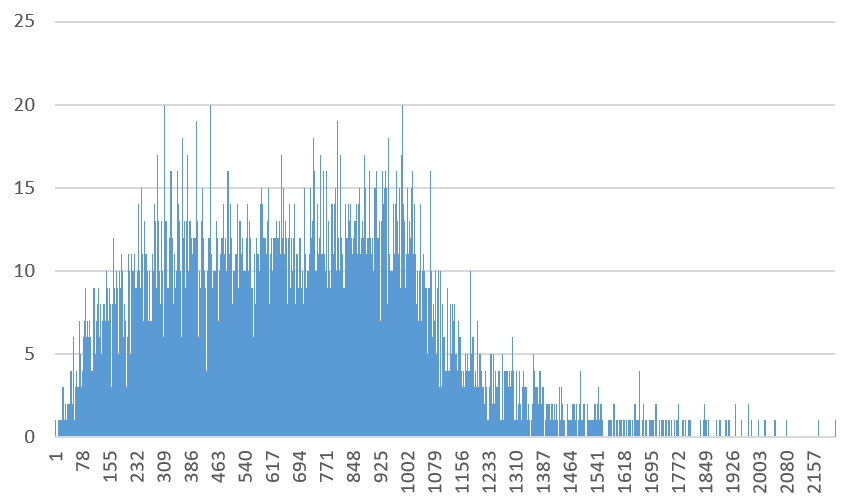
\includegraphics[width=0.7\textwidth]{figures/images/numberGenerator/overlapped.png}\label{fig:overlappedDistExample}
\end{figure}

Figure~\ref{fig:overlappedDistExample} looks completely different from figure~\ref{fig:mixedDistExample}.
No value is generated more than 20 times as opposed to the maximum amount of 350 for the mixed distribution.
In this figure no distribution is clearly visible.

The used distributions were \textasciitilde$U(1,49999)$, \textasciitilde$B(10000,0.1)$, \textasciitilde$Geo(0.001)$, powerlaw distribution with $\beta=-1.25$.
\subsection{RLS Comparison}
The following table lists the results for the RLS for inputs that are chosen from a powerlaw distribution with $\beta=-2.75$.


\makebox[\linewidth]{
\begin{tabular}{lp{3cm}p{6cm}p{6cm}}
\begin{tabular}[h]{cccccccc}
algo type&            \RLSN&     \RLSR&     \RLSR&     \RLSN&     \RLSR&     \RLSN&       RLS\\
algo param&             b=2&       s=3&       s=4&       b=3&       s=2&       b=4&         -\\
avg mut/change&       2.000&     1.996&     2.476&     3.000&     1.502&     4.000&     1.000\\
avg mut/step&         2.000&     2.000&     2.500&     3.000&     1.500&     4.000&     1.000\\
\hline
total avg count&     83,118&   104,748&   105,513&   112,223&   114,486&   121,927& 2,443,567\\
avg eval count&      83,118&   104,748&   105,513&   112,223&   114,486&   121,927&    45,834\\
max eval count&     778,110& 1,453,252&   898,974& 1,377,471&   915,268&   816,633&   485,275\\
min eval count&         197&       126&        45&       212&       271&       155&       128\\
\hline
fail ratio&           0.000&     0.000&     0.000&     0.000&     0.000&     0.000&     0.447\\
avg fail dif&             -&         -&         -&         -&         -&         -&         1\\
\end{tabular}
\end{tabular}
}


For these inputs the variants of the RLS perform differently to the binomial input.
The only similarity is the RLS being the worst as the RLS is the only algorithm that did not find an optimal solution for every input.
If the RLS did find an optimal solution in those 5 cases it would instead be the best RLS variant.
The other algorithms are ranked by the probability of flipping only one bit.
This means at first the three RLS-R variants from 2 to 3 to 4 and then the same for the RLS-N variants.
So it does seem like moving mostly one element at once is better for the geometric input in comparison to two elements for the binomial distribution.
In the 5 cases where the RLS did not find an optimal solution it was most likely stuck in a local optimum.

\subsection{(1+1) EA Comparison}
The first table again shows the results for parameter $\beta=-2.75$

\makebox[\linewidth]{
\begin{tabular}{lp{3cm}p{6cm}p{6cm}}
\begin{tabular}[h]{ccccccccc}
algo type&          (1+1) EA&   (1+1) EA&   (1+1) EA&   (1+1) EA&      (1+1) EA&   (1+1) EA&   (1+1) EA&   (1+1) EA\\
algo param&           3/n&     4/n&     2/n&     5/n&       -&    10/n&    50/n&   100/n\\
avg mut/change&     3.101&   3.968&   2.343&   4.859&   1.698&   9.732&  49.544&  99.494\\
avg mut/step&       2.999&   4.003&   2.002&   4.999&   1.001&   9.998&  49.998&  99.997\\
\hline
total avg count&      646&     701&     706&     857&   1,123&   1,508&   8,175&  15,485\\
avg eval count&       646&     701&     706&     857&   1,123&   1,508&   8,175&  15,485\\
max eval count&     5,346&   5,692&   3,415&   5,572&   7,001&  12,112&  52,831& 145,269\\
min eval count&        23&       4&      30&       9&      23&      14&      27&      69\\
\hline
fails&                  0&       0&       0&       0&       0&       0&       0&       0\\
fail ratio&         0.000&   0.000&   0.000&   0.000&   0.000&   0.000&   0.000&   0.000\\
avg fail dif&           -&       -&       -&       -&       -&       -&       -&       -\\
\end{tabular}
\end{tabular}
}


For the EA the result is also the inversion of the results for the OneMax equivalent.
The higher the mutation rate the better at least up to $n\le100$.
From mutation rate $p_m\le3/n$ the algorithm reaches the worst case at least once in 1000 runs.
If the algorithm did not manage to find an optimal solution the fitness was always the same.
So there was no run where any algorithm neither found a global nor the local optimum.
\subsection{pmut Comparison}
The first table again shows the results for parameter $\beta=-2.75$

\makebox[\linewidth]{
\scriptsize
\begin{tabular}{lp{3cm}p{6cm}p{6cm}}
\begin{tabular}[h]{m{2.5cm}m{0,40cm}m{0,40cm}m{0,40cm}m{0,40cm}m{0,40cm}m{0,40cm}m{0,40cm}m{0,40cm}m{0,40cm}m{0,40cm}m{0,40cm}m{0,40cm}m{0,40cm}m{0,40cm}m{0,40cm}m{0,40cm}m{0,40cm}m{0,40cm}}
\multicolumn{1}{c}{algo type}&\multicolumn{2}{c}{            pmut}&\multicolumn{2}{c}{     pmut}&\multicolumn{2}{c}{     pmut}&\multicolumn{2}{c}{     pmut}&\multicolumn{2}{c}{     pmut}&\multicolumn{2}{c}{     pmut}&\multicolumn{2}{c}{     pmut}&\multicolumn{2}{c}{     pmut}&\multicolumn{2}{c}{     pmut}\\
\multicolumn{1}{c}{algo param}&\multicolumn{2}{c}{           3.25}&\multicolumn{2}{c}{     3.00}&\multicolumn{2}{c}{     2.75}&\multicolumn{2}{c}{     2.50}&\multicolumn{2}{c}{     2.25}&\multicolumn{2}{c}{     2.00}&\multicolumn{2}{c}{     1.75}&\multicolumn{2}{c}{     1.50}&\multicolumn{2}{c}{     1.25}\\
\multicolumn{1}{c}{avg mut/change}&\multicolumn{2}{c}{      1.583}&\multicolumn{2}{c}{    1.737}&\multicolumn{2}{c}{    2.002}&\multicolumn{2}{c}{    2.423}&\multicolumn{2}{c}{    3.303}&\multicolumn{2}{c}{    5.830}&\multicolumn{2}{c}{   12.519}&\multicolumn{2}{c}{   30.910}&\multicolumn{2}{c}{   73.182}\\
\multicolumn{1}{c}{avg mut/step}&\multicolumn{2}{c}{        1.729}&\multicolumn{2}{c}{    1.934}&\multicolumn{2}{c}{    2.274}&\multicolumn{2}{c}{    2.895}&\multicolumn{2}{c}{    4.360}&\multicolumn{2}{c}{    8.452}&\multicolumn{2}{c}{   22.278}&\multicolumn{2}{c}{   70.532}&\multicolumn{2}{c}{  224.421}\\
\hline
\multicolumn{1}{c}{avg eval count}&\multicolumn{2}{c}{        540}&\multicolumn{2}{c}{      569}&\multicolumn{2}{c}{      594}&\multicolumn{2}{c}{      641}&\multicolumn{2}{c}{      712}&\multicolumn{2}{c}{      808}&\multicolumn{2}{c}{      967}&\multicolumn{2}{c}{    1,285}&\multicolumn{2}{c}{    2,081}\\
\multicolumn{1}{c}{max eval count}&\multicolumn{2}{c}{      3,110}&\multicolumn{2}{c}{    2,891}&\multicolumn{2}{c}{    3,504}&\multicolumn{2}{c}{    3,896}&\multicolumn{2}{c}{    5,152}&\multicolumn{2}{c}{    4,274}&\multicolumn{2}{c}{    5,610}&\multicolumn{2}{c}{    6,190}&\multicolumn{2}{c}{   14,984}\\
\multicolumn{1}{c}{min eval count}&\multicolumn{2}{c}{         22}&\multicolumn{2}{c}{        9}&\multicolumn{2}{c}{       36}&\multicolumn{2}{c}{       25}&\multicolumn{2}{c}{       28}&\multicolumn{2}{c}{       27}&\multicolumn{2}{c}{       27}&\multicolumn{2}{c}{       13}&\multicolumn{2}{c}{       33}\\
\hline
\multicolumn{1}{c}{fail ratio}&\multicolumn{2}{c}{          0.000}&\multicolumn{2}{c}{    0.000}&\multicolumn{2}{c}{    0.000}&\multicolumn{2}{c}{    0.000}&\multicolumn{2}{c}{    0.000}&\multicolumn{2}{c}{    0.000}&\multicolumn{2}{c}{    0.000}&\multicolumn{2}{c}{    0.000}&\multicolumn{2}{c}{    0.000}\\
\hline
\multicolumn{1}{c}{p-value}&&\multicolumn{2}{c}{0.0000}&\multicolumn{2}{c}{0.0000}&\multicolumn{2}{c}{0.0000}&\multicolumn{2}{c}{0.0000}&\multicolumn{2}{c}{0.0000}&\multicolumn{2}{c}{0.0000}&\multicolumn{2}{c}{0.0000}&\multicolumn{2}{c}{0.0000}\\
&&&&&&&&&&&&&&&&&&\end{tabular}
\end{tabular}
}


The ideal value for $\beta$ seems to be around -1.75 as the runtime increases for the two neighbour values.
Even the worst value still manages find an optimal solution within double the time of the best value.
The importance of the parameter is therefore not as important as for other inputs.
\subsection{Comparison of the best variants}
The first table again shows the results for parameter $\beta=-2.75$

\makebox[\linewidth]{
\begin{tabular}{lp{3cm}p{6cm}p{6cm}}
\begin{tabular}[h]{cccc}
algo type&            RLS&    pmut&      EA\\
algo param&             -&    3.25&       -\\
avg mut/change&     1.000&   1.287&   1.272\\
avg mut/step&       1.000&   1.729&   1.000\\
\hline
avg eval count&    91,171& 143,121& 231,082\\
max eval count&   153,143& 227,737& 446,942\\
min eval count&    65,783&  93,602& 165,818\\
\hline
fail ratio&         0.000&   0.000&   0.000\\
\end{tabular}
\end{tabular}
}


The results for this experiment are as expected.
All three algorithms find the optimal value within the time limit.
The RLS performs better than the (1+1) EA because it does only single bit flips.
The $pmut_{-3.25}$ perform better than the standard (1+1) EA although flipping more bits on average.
This is most likely cause by the few steps where $pmut$ flips many bits which increase the average.
But $pmut$ most likely chooses to flip only one bit more often as the (1+1) EA.

TODO insert comparison with multiple values of n.
\section{Multiple distributions mixed \& overlapped}
This input is similar to the mixed input from the last subsection.
For this distribution the values are not chosen uniform random from one of the base distributions, but instead a value from every distribution is chosen and added together.
Hence the name overlapped distribution.
For this input the step limit was increased to $100\cdot n \ln n$.
The comparison with the step limit $10\cdot n \ln(n)$ is contained in the last subsubsection which compares the best variants.

\begin{figure}[h]
      \caption{Distribution of an overlapped input with \textasciitilde$U(1,999)$, \textasciitilde$B(1000,0.1)$, \textasciitilde$Geo(0.01)$, powerlaw dist with $\beta=-1.25$}
      \centering
      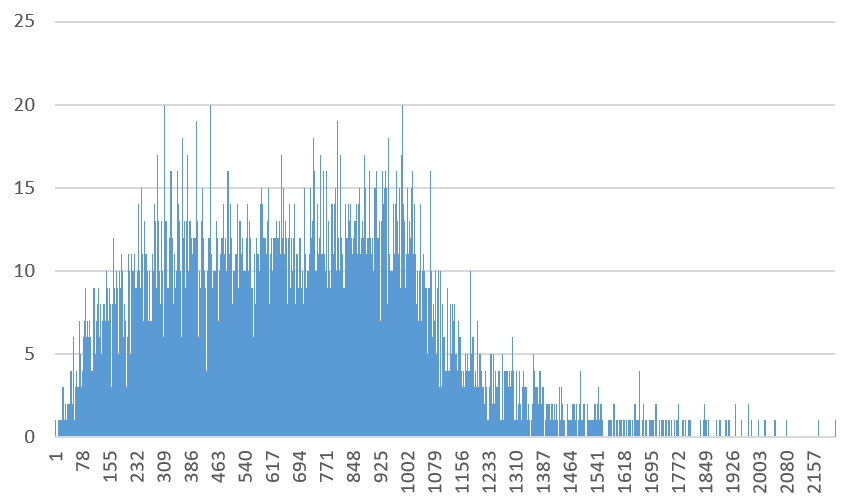
\includegraphics[width=0.7\textwidth]{figures/images/numberGenerator/overlapped.png}\label{fig:overlappedDistExample}
\end{figure}

Figure~\ref{fig:overlappedDistExample} looks completely different from figure~\ref{fig:mixedDistExample}.
No value is generated more than 20 times as opposed to the maximum amount of 350 for the mixed distribution.
In this figure no distribution is clearly visible.

The used distributions were \textasciitilde$U(1,49999)$, \textasciitilde$B(10000,0.1)$, \textasciitilde$Geo(0.001)$, powerlaw distribution with $\beta=-1.25$.
\subsection{RLS Comparison}
The following table lists the results for the RLS for inputs that are chosen from a powerlaw distribution with $\beta=-2.75$.


\makebox[\linewidth]{
\begin{tabular}{lp{3cm}p{6cm}p{6cm}}
\begin{tabular}[h]{cccccccc}
algo type&            \RLSN&     \RLSR&     \RLSR&     \RLSN&     \RLSR&     \RLSN&       RLS\\
algo param&             b=2&       s=3&       s=4&       b=3&       s=2&       b=4&         -\\
avg mut/change&       2.000&     1.996&     2.476&     3.000&     1.502&     4.000&     1.000\\
avg mut/step&         2.000&     2.000&     2.500&     3.000&     1.500&     4.000&     1.000\\
\hline
total avg count&     83,118&   104,748&   105,513&   112,223&   114,486&   121,927& 2,443,567\\
avg eval count&      83,118&   104,748&   105,513&   112,223&   114,486&   121,927&    45,834\\
max eval count&     778,110& 1,453,252&   898,974& 1,377,471&   915,268&   816,633&   485,275\\
min eval count&         197&       126&        45&       212&       271&       155&       128\\
\hline
fail ratio&           0.000&     0.000&     0.000&     0.000&     0.000&     0.000&     0.447\\
avg fail dif&             -&         -&         -&         -&         -&         -&         1\\
\end{tabular}
\end{tabular}
}


For these inputs the variants of the RLS perform differently to the binomial input.
The only similarity is the RLS being the worst as the RLS is the only algorithm that did not find an optimal solution for every input.
If the RLS did find an optimal solution in those 5 cases it would instead be the best RLS variant.
The other algorithms are ranked by the probability of flipping only one bit.
This means at first the three RLS-R variants from 2 to 3 to 4 and then the same for the RLS-N variants.
So it does seem like moving mostly one element at once is better for the geometric input in comparison to two elements for the binomial distribution.
In the 5 cases where the RLS did not find an optimal solution it was most likely stuck in a local optimum.

\subsection{(1+1) EA Comparison}
The first table again shows the results for parameter $\beta=-2.75$

\makebox[\linewidth]{
\begin{tabular}{lp{3cm}p{6cm}p{6cm}}
\begin{tabular}[h]{ccccccccc}
algo type&          (1+1) EA&   (1+1) EA&   (1+1) EA&   (1+1) EA&      (1+1) EA&   (1+1) EA&   (1+1) EA&   (1+1) EA\\
algo param&           3/n&     4/n&     2/n&     5/n&       -&    10/n&    50/n&   100/n\\
avg mut/change&     3.101&   3.968&   2.343&   4.859&   1.698&   9.732&  49.544&  99.494\\
avg mut/step&       2.999&   4.003&   2.002&   4.999&   1.001&   9.998&  49.998&  99.997\\
\hline
total avg count&      646&     701&     706&     857&   1,123&   1,508&   8,175&  15,485\\
avg eval count&       646&     701&     706&     857&   1,123&   1,508&   8,175&  15,485\\
max eval count&     5,346&   5,692&   3,415&   5,572&   7,001&  12,112&  52,831& 145,269\\
min eval count&        23&       4&      30&       9&      23&      14&      27&      69\\
\hline
fails&                  0&       0&       0&       0&       0&       0&       0&       0\\
fail ratio&         0.000&   0.000&   0.000&   0.000&   0.000&   0.000&   0.000&   0.000\\
avg fail dif&           -&       -&       -&       -&       -&       -&       -&       -\\
\end{tabular}
\end{tabular}
}


For the EA the result is also the inversion of the results for the OneMax equivalent.
The higher the mutation rate the better at least up to $n\le100$.
From mutation rate $p_m\le3/n$ the algorithm reaches the worst case at least once in 1000 runs.
If the algorithm did not manage to find an optimal solution the fitness was always the same.
So there was no run where any algorithm neither found a global nor the local optimum.
\subsection{pmut Comparison}
The first table again shows the results for parameter $\beta=-2.75$

\makebox[\linewidth]{
\scriptsize
\begin{tabular}{lp{3cm}p{6cm}p{6cm}}
\begin{tabular}[h]{m{2.5cm}m{0,40cm}m{0,40cm}m{0,40cm}m{0,40cm}m{0,40cm}m{0,40cm}m{0,40cm}m{0,40cm}m{0,40cm}m{0,40cm}m{0,40cm}m{0,40cm}m{0,40cm}m{0,40cm}m{0,40cm}m{0,40cm}m{0,40cm}m{0,40cm}}
\multicolumn{1}{c}{algo type}&\multicolumn{2}{c}{            pmut}&\multicolumn{2}{c}{     pmut}&\multicolumn{2}{c}{     pmut}&\multicolumn{2}{c}{     pmut}&\multicolumn{2}{c}{     pmut}&\multicolumn{2}{c}{     pmut}&\multicolumn{2}{c}{     pmut}&\multicolumn{2}{c}{     pmut}&\multicolumn{2}{c}{     pmut}\\
\multicolumn{1}{c}{algo param}&\multicolumn{2}{c}{           3.25}&\multicolumn{2}{c}{     3.00}&\multicolumn{2}{c}{     2.75}&\multicolumn{2}{c}{     2.50}&\multicolumn{2}{c}{     2.25}&\multicolumn{2}{c}{     2.00}&\multicolumn{2}{c}{     1.75}&\multicolumn{2}{c}{     1.50}&\multicolumn{2}{c}{     1.25}\\
\multicolumn{1}{c}{avg mut/change}&\multicolumn{2}{c}{      1.583}&\multicolumn{2}{c}{    1.737}&\multicolumn{2}{c}{    2.002}&\multicolumn{2}{c}{    2.423}&\multicolumn{2}{c}{    3.303}&\multicolumn{2}{c}{    5.830}&\multicolumn{2}{c}{   12.519}&\multicolumn{2}{c}{   30.910}&\multicolumn{2}{c}{   73.182}\\
\multicolumn{1}{c}{avg mut/step}&\multicolumn{2}{c}{        1.729}&\multicolumn{2}{c}{    1.934}&\multicolumn{2}{c}{    2.274}&\multicolumn{2}{c}{    2.895}&\multicolumn{2}{c}{    4.360}&\multicolumn{2}{c}{    8.452}&\multicolumn{2}{c}{   22.278}&\multicolumn{2}{c}{   70.532}&\multicolumn{2}{c}{  224.421}\\
\hline
\multicolumn{1}{c}{avg eval count}&\multicolumn{2}{c}{        540}&\multicolumn{2}{c}{      569}&\multicolumn{2}{c}{      594}&\multicolumn{2}{c}{      641}&\multicolumn{2}{c}{      712}&\multicolumn{2}{c}{      808}&\multicolumn{2}{c}{      967}&\multicolumn{2}{c}{    1,285}&\multicolumn{2}{c}{    2,081}\\
\multicolumn{1}{c}{max eval count}&\multicolumn{2}{c}{      3,110}&\multicolumn{2}{c}{    2,891}&\multicolumn{2}{c}{    3,504}&\multicolumn{2}{c}{    3,896}&\multicolumn{2}{c}{    5,152}&\multicolumn{2}{c}{    4,274}&\multicolumn{2}{c}{    5,610}&\multicolumn{2}{c}{    6,190}&\multicolumn{2}{c}{   14,984}\\
\multicolumn{1}{c}{min eval count}&\multicolumn{2}{c}{         22}&\multicolumn{2}{c}{        9}&\multicolumn{2}{c}{       36}&\multicolumn{2}{c}{       25}&\multicolumn{2}{c}{       28}&\multicolumn{2}{c}{       27}&\multicolumn{2}{c}{       27}&\multicolumn{2}{c}{       13}&\multicolumn{2}{c}{       33}\\
\hline
\multicolumn{1}{c}{fail ratio}&\multicolumn{2}{c}{          0.000}&\multicolumn{2}{c}{    0.000}&\multicolumn{2}{c}{    0.000}&\multicolumn{2}{c}{    0.000}&\multicolumn{2}{c}{    0.000}&\multicolumn{2}{c}{    0.000}&\multicolumn{2}{c}{    0.000}&\multicolumn{2}{c}{    0.000}&\multicolumn{2}{c}{    0.000}\\
\hline
\multicolumn{1}{c}{p-value}&&\multicolumn{2}{c}{0.0000}&\multicolumn{2}{c}{0.0000}&\multicolumn{2}{c}{0.0000}&\multicolumn{2}{c}{0.0000}&\multicolumn{2}{c}{0.0000}&\multicolumn{2}{c}{0.0000}&\multicolumn{2}{c}{0.0000}&\multicolumn{2}{c}{0.0000}\\
&&&&&&&&&&&&&&&&&&\end{tabular}
\end{tabular}
}


The ideal value for $\beta$ seems to be around -1.75 as the runtime increases for the two neighbour values.
Even the worst value still manages find an optimal solution within double the time of the best value.
The importance of the parameter is therefore not as important as for other inputs.
\subsection{Comparison of the best variants}
The first table again shows the results for parameter $\beta=-2.75$

\makebox[\linewidth]{
\begin{tabular}{lp{3cm}p{6cm}p{6cm}}
\begin{tabular}[h]{cccc}
algo type&            RLS&    pmut&      EA\\
algo param&             -&    3.25&       -\\
avg mut/change&     1.000&   1.287&   1.272\\
avg mut/step&       1.000&   1.729&   1.000\\
\hline
avg eval count&    91,171& 143,121& 231,082\\
max eval count&   153,143& 227,737& 446,942\\
min eval count&    65,783&  93,602& 165,818\\
\hline
fail ratio&         0.000&   0.000&   0.000\\
\end{tabular}
\end{tabular}
}


The results for this experiment are as expected.
All three algorithms find the optimal value within the time limit.
The RLS performs better than the (1+1) EA because it does only single bit flips.
The $pmut_{-3.25}$ perform better than the standard (1+1) EA although flipping more bits on average.
This is most likely cause by the few steps where $pmut$ flips many bits which increase the average.
But $pmut$ most likely chooses to flip only one bit more often as the (1+1) EA.

TODO insert comparison with multiple values of n.


\subsection{Conclusion of empirical results}
